% ####################################################################

\setcounter{chapter}{3}
\chapter{Multi-level selection\is{multi-level selection} and language systematicity\is{systematicity}}
\label{c:experiment1}

The baseline experiments of the previous chapter looked at how analog\is{analogy}y could be exploited for the generalization of case marker\is{case!case marking}s for covering semantic roles. The experiments focused on the development of these semantic roles in isolation of each other in order to identify the diagnostic\is{learning strategies!diagnostics}s, repair\is{learning strategies!repair strategies}s and alignment strateg\is{alignment strategy}ies that make the emergence\is{formation} of such roles possible. However, the behaviour and functionality of case marker\is{case!case marking}s can only be fully understood when they are studied in relation to the other elements in their linguistic context. In other words: case marker\is{case!case marking}s have to be investigated in relation to the patterns in which they occur. This chapter therefore presents experiments in which case marker\is{case!case marking}s can be combined in larger patterns.

The next section first gives a brief overview of pattern formation\is{formation}\is{pattern formation} in language and operationalizes one strategy of pattern formation\is{pattern formation} in the form of diagnostic\is{learning strategies!diagnostics}s, repair\is{learning strategies!repair strategies}s and alignment strateg\is{alignment strategy}ies. Section \ref{s:pattern-exp-1} implements this operationalization and shows that the `systematicity\is{systematicity}' of the artificial languages gets lost once smaller linguistic units are starting to combine into larger patterns. In this section I will also briefly discuss other experiments in the field in which the problem of systematicity\is{systematicity} occurs but is either overlooked or misinterpreted by the experimenter. The next section then presents the results of another experiment that uses the more complex alignment strateg\is{alignment strategy}y of multi-level selection\is{multi-level selection} to overcome this problem. Three variation\is{variation}s of multi-level selection\is{multi-level selection} are implemented and compared to each other in terms of systematicity\is{systematicity} and coherence. The insights of these experiments are ported to experiments involving analog\is{analogy}y and the formation\is{formation} of semantic roles in section \ref{s:pattern-exp-3}. Section \ref{s:pattern-exp-4} finally offers a first step towards simulations involving the formation\is{formation} of syntactic cases (corresponding to stage 3 in section \ref{s:stage3}). Even though stage 3 is not fully accomplished yet, this section offers a clear idea of the work that needs to be undertaken in order to form syntactic cases.

\section{Pattern formation}
\label{s:pattern-formation}

One crucial aspect of grammaticalization (see Martin Haspelmath's definition in section \ref{s:assumptions}) is the evolution towards tighter structures and a lesser degree of freedom. For example, lexical items develop into more grammatical items and become part of (larger) constructions. Within these constructions or patterns, the freedom of the individual parts is restricted and depends on the pattern as a whole. This would explain why for example an allative\is{case!allative} case marker\is{case!case marking} only makes sense in a motion-pattern. However, linguistic items that become part of a larger construction may still have a life on their own in their original sense, a phenomenon traditionally known as `layering\is{synchron\is{synchronic}ic layering}' \citep[124--126]{hopper93grammaticalization}. For example the preposition\is{preposition} {\em like} can still be used for indicating similarity while at the same time it can be used as a marker\is{case!case marking} for introducing reported speech:

\ea
She looks nothing {\em like} her father.
\item And he was {\em like} ``Oh that is so not true!''
\z

In the following subsection I will briefly touch upon some phenomena of grammaticalization involving pattern formation\is{pattern formation} and offer an analysis which is somewhat different from the traditional linguistic approach. I will support my analysis through other examples of patterns and idiom\is{idiom}s in language. In the next subsection, I will then offer an operationalization of my analysis in terms of diagnostic\is{learning strategies!diagnostics}s and repair\is{learning strategies!repair strategies} strategies for the artificial agents that will be used in the experiments in this chapter.



\subsection{Pattern formation\is{pattern formation} in language}

A very good example of the development of a lexical item into a part of a grammatical structure can be found in French\is{French} negation\is{negation}. Traditionally, the development of negation\is{negation} particles (also known as `Jespersen's cycle\is{Jespersen's cycle}') is defined in terms of a cycle of reanalysis\is{reanalysis} -- analog\is{analogy}y (generalization) -- reanalysis\is{reanalysis} \cite[65--66]{hopper93grammaticalization}:

\begin{enumerate}  \item[1.]   Negation in French\is{French} originally only involved {\em ne} before the verb\is{verb}:
\end{enumerate}
 



\ea
\gll Il ne va.\\
he {\textsc{neg}} go.3{\sg}.{\prs}\\
\glt `He doesn't go.'\\
\z

 \begin{enumerate}  \item[2.]   In the context of motion verb\is{verb}s, {\em ne} could optionally be reinforc\is{reinforcement}ed by the noun\is{noun} {\em pas} `step':
 \end{enumerate}


\ea
\gll Il ne va (pas).\\
he {\textsc{neg}} go.3{\sg}.{\prs} (step)\\
\glt `He doesn't go (a step).'\\
\z
\begin{enumerate}  \item[3.]  The word {\em pas} is reanalyzed as a negator particle in the construction [{\em ne} Vmotion {\em pas}];
\end{enumerate}

\begin{enumerate}  \item[4.]   The particle {\em pas} is exten\is{extension}ded analog\is{analogy}ically to non-motion verb\is{verb}s as well:
\end{enumerate}

 

\ea
\gll Il ne sait pas.\\
he {\textsc{neg}} know.3{\sg}.{\prs} {\textsc{neg}}\\
\glt `He doesn't know.'\\
\z


\begin{enumerate}  \item[5.]  The particle {\em pas} is then reanalyzed as an obligatory part of the construction [{\em ne} V {\em pas}];
\end{enumerate}


\begin{enumerate}  \item[6.]  In spoken French\is{French}, {\em ne} is reanalyzed to become optional and is eventually lost:
\end{enumerate}
 
\ea
\gll Il sait pas.\\
he know.3{\sg}.{\prs} {\textsc{neg}}\\
\glt `He doesn't know.'\\
\z 

\subsubsection{Reanalysis versus pattern formation\is{formation}\is{pattern formation}}
 Reanalysis is essentially a hearer-based analysis of this developmental cycle in which the hearer interprets the underlying structure of an utterance in another way than was intended by the speaker. Reanalysis is traditionally understood as {\em ``change in the structure of an expression or class of expressions that does not involve any immediate or intrinsic modification of its surface manifestation''} \citep[58]{langacker77syntactic}. Even though reanalysis\is{reanalysis} is a plausible mechanism for step 3, its main problem is that it is invisible from the outside. \citet{hopper93grammaticalization} write that for {\em ``the French\is{French} negator {\em pas}, we would not know that reanalysis\is{reanalysis} had taken place at stage [3] without the evidence of the working generalization at stage [4]''} (p. 66). As \citet{haspelmath98does} points out, however, this means that reanalysis\is{reanalysis} cannot explain how the new use of {\em pas} got propagat\is{propagation}ed and accepted in the speech community\is{speech population} unless all speakers are assumed to make the same reanalysis\is{reanalysis} at roughly the same time, which is very implausible. As I will explain more thoroughly in section \ref{s:actualization}, reanalysis\is{reanalysis} needs to be accompanied by other mechanisms in order to account for the empirical data.

I propose a different and simpler mechanism for step 3 that is in line with the general approach of usage-based model\is{usage-based model}s of language: pattern formation\is{formation}\is{pattern formation}. If a certain group of words occur frequently enough together, they are stored as a new unit in the linguistic inventor\is{linguistic inventory}y. This means that the language user now knows two {\bfseries competing} constructions in the case of motion verb\is{verb}s: [{\em ne} V] and [{\em ne} Vmotion {\em pas}]. This approach of pattern formation\is{pattern formation} may seem redundant from the point of view of inventory size, but it may optimize linguistic processing because a pattern is a `pre-compiled' chunk that is readily available for use, whereas otherwise the language user needs to compose the structure over and over again. Since pattern formation\is{pattern formation} is a relatively `simple' operation for optimizing processing, we can assume within a usage-based model\is{usage-based model} that most language users will do this spontaneously for all recurrent patterns in the language as opposed to a collective operation of reanalysis\is{reanalysis}. Once a pattern is stored in memory, it can start a life on its own and diverge from its original usage. Steps 1--5 in the negation\is{negation} cycle can thus be reinterpreted as follows in a more speaker-based analysis:


\begin{enumerate}  \item[1.]  Negation in French\is{French} originally only involved {\em ne} before the verb\is{verb}:
\end{enumerate}
 
\ea
\gll Il ne va.\\
he {\textsc{neg}} go.3{\sg}.{\prs}\\
\glt `He doesn't go.'\\
\z

\begin{enumerate}  \item[2.]  The speakers of French\is{French} start to reinforc\is{reinforcement}e the negation\is{negation} particle {\em ne} in some situations to put more emphasis on the negation\is{negation} or to solve communicative problems. In the context of motion verb\is{verb}s, the reinforc\is{reinforcement}ement is achieved through the noun\is{noun} {\em pas} `step', whereas in other contexts such as verb\is{verb}s of visual perception, negation\is{negation} is reinforc\is{reinforcement}ed through {\em point} `point':

\end{enumerate}
  
\ea
\gll Il ne va (pas).\\
he {\textsc{neg}} go.3{\sg}.{\prs} (step)\\
\glt `He doesn't go (a step).'\\

\item
\gll Il ne voit (point).\\
he {\textsc{neg}} see.3{\sg}.{\prs} (point)\\
\glt `He doesn't see (a point).'\\
\z

\begin{enumerate}  \item[3.]   The frequent use of these reinforc\is{reinforcement}ement noun\is{noun}s leads to the creation of readily available patterns which co-exist\is{co-existence} (and compete with) the standard negation\is{negation} construction;
\end{enumerate}


\begin{enumerate}  \item[4.]  The new patterns are exten\is{extension}ded analog\is{analogy}ically to non-motion verb\is{verb}s as well and start to compete with each other and with the old negation\is{negation} construction for becoming the new default negation\is{negation};

\end{enumerate}



\begin{enumerate}  \item[5.]  The construction [{\em ne} V {\em pas}] wins the competit\is{competition}ion and becomes the new default construction for negation\is{negation}. Other competit\is{competition}ors using different particles either disappear or take up their own semantic niche ({\em ne ... point} `nothing' (old-fashioned), {\em ne ... plus} `no more', {\em ne ... rien} `nothing', {\em ne ... jamais} `never', {\em ne ... gu\`{e}re} `almost nothing', etc.). The old negation\is{negation} construction gets lost except for some archaic uses in writing.
\end{enumerate}

 

\subsubsection{Idioms}
 Evidence for pattern formation\is{pattern formation} as opposed to reanalysis\is{reanalysis} can be found in idiom\is{idiom}s. Idiomatic expressions have always been problematic for traditional linguistic theories that take a modular approach to language and assume a sharp distinction between convention\is{convention}al-lexical items and systematic-syntactic rules. Faced with such problematic issues, usage-based model\is{usage-based model}s and particularly construction grammars {\em ``grew out of a concern to find a place for idiom\is{idiom}atic expressions in the speaker's knowledge of a grammar of their language''} \citep[225]{croft04cognitive}. Idioms range from highly idiom\is{idiom}atic expressions to more schematic constructions \citep[][chapter 9]{croft04cognitive}:

\ea
by and large; no can do; be that as it may; make believe; so far so good
\item kick the bucket; pull a fast one; spill the beans
\item to answer the door; wide awake; bright red; to blow one's nose
\item the bigger the better; the louder you shout, the sooner they will serve you
%\item what's a girl like you doing in a place like this
\z

No theory of grammaticalization that I am aware of explains idiom\is{idiom}s such as {\em so far so good} or {\em by and large} in terms of reanalysis\is{reanalysis} of the words that make up the idiom\is{idiom}. Similarly, compound noun\is{noun}s are given their own lexical entry rather than introducing a notion of `synchron\is{synchronic}ic layering\is{synchron\is{synchronic}ic layering}' \citep[124--126]{hopper93grammaticalization} over the original words caused by reanalysis\is{reanalysis}. Also pattern formation\is{formation}\is{pattern formation} on other levels of language (e.g. reoccurring syllables, morphemes, etc.) are never treated as synchron\is{synchronic}ic layers on top of one entry in the linguistic inventor\is{linguistic inventory}y. Reanalysis is therefore used in an ad-hoc way, or as \citet{haspelmath98does} writes, {\em ``as one pleases''} (p. 341).

By taking pattern formation\is{formation}\is{pattern formation} seriously, meaning that many redundant copies exist in memory, a simpler alternative exists for the ad-hoc mechanism of reanalysis\is{reanalysis}. Just as there is no reason for differentiating `core case marker\is{case!case marking}s' from `peripheral semantic case marker\is{case!case marking}s' (see section \ref{s:stage4}), the language user makes no difference between fully idiom\is{idiom}atic expressions such as {\em by and large} and more grammatical constructions such as [{\em ne} ... {\em pas}]. The only difference between them is that the more schematic constructions were exten\is{extension}ded and generaliz\is{generalization}ed to new uses whereas the more idiom\is{idiom}atic expressions remained unchanged depending on communicative needs in language use and frequency\is{frequency} effects. This usage-based approach\is{usage-based model} naturally leads to the continuum\is{syntax-lexicon continuum} of linguistic items as observed in natural languages.

One problem with the alternative hypothesis is that it is invisible from the outside just like reanalysis\is{reanalysis} is. This is where computational models can prove their worth: they can {\bfseries demonstrate} the consequences of each alternative hypothesis and show what kind of cognitive apparatus is needed for both. Additional evidence can then be gathered from other disciplines such as psycholinguistics to determine which cognitive architecture is most plausible. So even though computational modeling cannot predict actual language change\is{language change}, they can demonstrate the effects of proposed mechanisms and help to fill in the blanks when there is a lack of empirical data.

\subsection{Operationalizing pattern formation\is{formation}\is{pattern formation}}
\label{s:operationalizing-patterns}

The above idea of pattern formation\is{formation}\is{pattern formation} needs to be implemented in terms of diagnostic\is{learning strategies!diagnostics}s and repair\is{learning strategies!repair strategies} strategies that make use of information that is locally available to the agents. Consider the reaction network\is{reaction network} of Figure \ref{f:reaction1} in which an agent used two constructions which subsequently license\is{license}d node-2 and node-3 in the network and which license\is{license}s the utterance {\em jack -bo push block -ka}:

\begin{figure}[htb]
\centerline{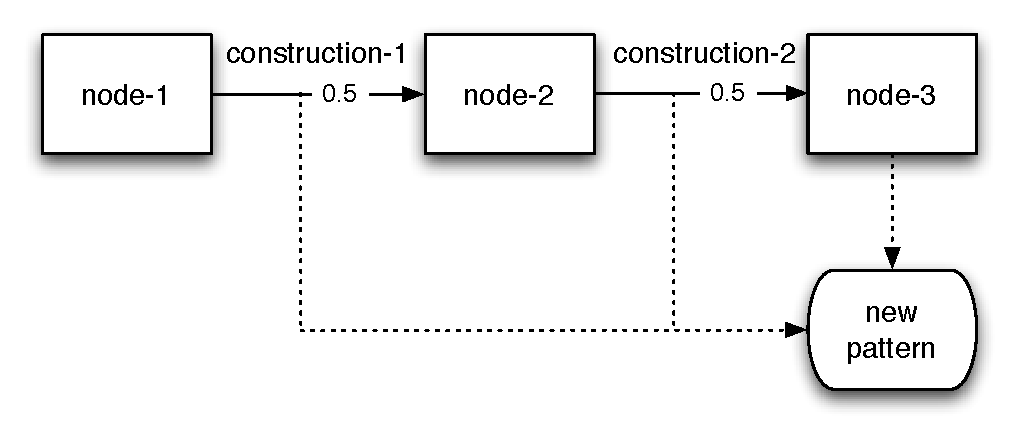
\includegraphics[width=0.8\textwidth]{Chapter4/figs/reaction1}}
  \caption[A reaction network\is{reaction network} as a source for pattern formation\is{formation}\is{pattern formation}]{An agent's reaction network\is{reaction network} is the source for pattern formation\is{pattern formation}. If the agents have to apply two constructions to license\is{license} an utterance (production) or a meaning (parsing), they will create a pattern based on the applied constructions. This pattern has the same functionality as the constructions but only requires one step.}
   \label{f:reaction1}
\end{figure}

Suppose that the agent is in production mode. In this case node-1 is the coupled feature structure\is{feature structure!coupled feature structure} which was license\is{license}d after unify\is{unify and merge}ing and merging the lexical entries for {\em jack, push} and {\em block}. Next, the speaker has to unify\is{unify and merge} and merge two constructions for marking the two participants of the push-event which license\is{license}s node-3. In a next step, which is not shown in the figure, the agent will unify\is{unify and merge} and merge the morphological rules. As indicated in the figure, this reaction network\is{reaction network} forms the basis for a new pattern (which will be construction-3). In principle this pattern should combine the entire reaction network\is{reaction network} including the lexical entries, but for convenience's sake the agents will only make a pattern which combines the functionality of constructions 1 and 2, as shown in Figure \ref{f:new-pattern}.
\begin{figure}[htb]
\centerline{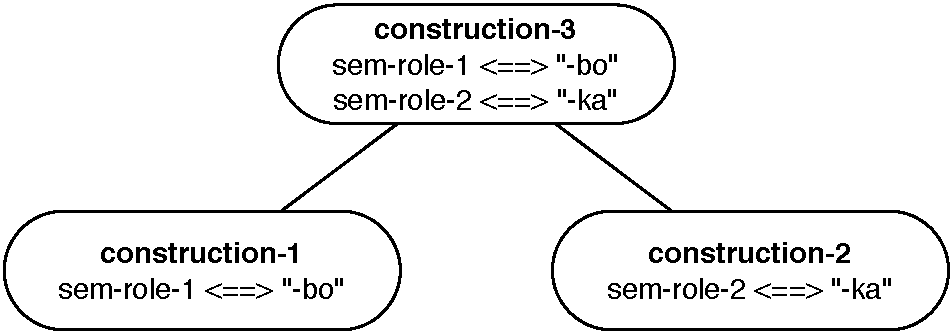
\includegraphics[width=0.8\textwidth]{Chapter4/figs/new-pattern}}
  \caption[A new pattern]{The two constructions that were used during processing are combined into a new construction. The agents keep a link between the new construction and the constructions that were used for creating it.}
   \label{f:new-pattern}
\end{figure}

The new construction is stored in the linguistic inventor\is{linguistic inventory}y with information about its origins: the agents keep a link between the new pattern and the constructions that were used for creating it. If the speaker has to produce the same meaning again, the new construction now forms an alternative path in the reaction network\is{reaction network}. The speaker will prefer this new path because it is faster in processing (one step can be skipped) and the links between the constructions can be used for giving priority to larger constructions if they unify\is{unify and merge} and merge. This new reaction network\is{reaction network} is illustrated in Figure \ref{f:reaction2}.
\begin{figure}[h]
\centerline{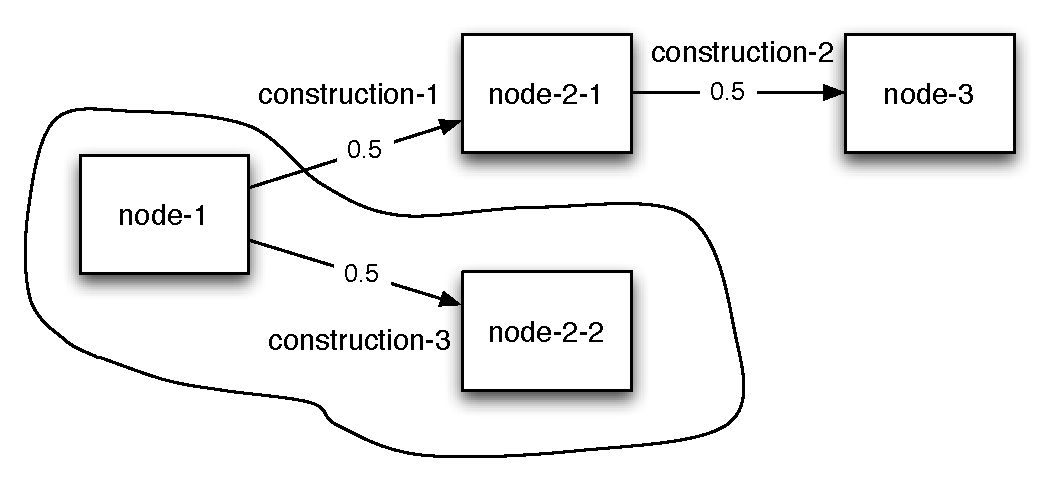
\includegraphics[width=0.8\textwidth]{Chapter4/figs/reaction2}}
  \caption[A reaction network\is{reaction network} with the new pattern]{The new construction now offers the agent an alternative path in the reaction network\is{reaction network}. Since the new pattern yields the same coupled feature structure\is{feature structure!coupled feature structure} as node-3 in only one step, it is faster and therefore preferred. The links between the three constructions are used to give larger patterns priority if they unify\is{unify and merge} and merge.}
   \label{f:reaction2}
\end{figure}

Apart from creating the new pattern, not much needs to be changed in the linguistic inventor\is{linguistic inventory}y apart from the fact that the agents have to link the new construction to the lexical entries that are compatible with it. The agents will not do this in one sweep but postpone this task until processing: lexical entries are only linked to the new construction instance by instance if this is required during a language game\is{language game}. The mechanism works entirely the same: the agent wants to unify\is{unify and merge} and merge two constructions and wants to optimize processing by creating a pattern. This time, however, no new pattern needs to be created because there is already one. The pattern thus exten\is{extension}ds its use to a new verb\is{verb} as well. The newly-made construction looks as follows:

\begin{lstlisting}
<Construction: construction-3
((?top-unit
   (sem-subunits (== ?unit-a ?unit-b ?unit-c)))
 (?unit-a
   (sem-frame (== (sem-role-1 ?unit-b ?obj-x)
                  (sem-role-2 ?unit-c ?obj-y))))
 (?unit-b
   (referent ?obj-x))
 (?unit-c
   (referent ?obj-y))
 ((J ?unit-b NIL)
   (sem-role sem-role-1))
 ((J ?unit-c NIL)
   (sem-role sem-role-2)))
<==>
((?top-unit
   (syn-subunits (== ?unit-a ?unit-b ?unit-c)))
 (?unit-a
   (syn-frame (== (syn-role-1 ?unit-b)
                  (syn-role-2 ?unit-c))))
 (?unit-b
   (syn-role syn-role-1))
 (?unit-c
   (syn-role syn-role-2)))>
\end{lstlisting}


\noindent To summarize, the agents are equipped with the following diagnostic\is{learning strategies!diagnostics} and repair\is{learning strategies!repair strategies} strategy in all the experiments in this chapter:

\begin{enumerate}
\item {\bfseries Diagnostic:} If two constructions are used together for licensing a node in the network, report an opportunity for optimizing processing (both for production and parsing);
\item {\bfseries Repair strategy:} If there is a problem of processing effort: 
\begin{enumerate}
\item If a larger construction already exists for the same mapping, create a link between the lexical entry and the construction;
\item Else combine the two constructions into a new construction and keep a link between them.
\end{enumerate}
\end{enumerate}

During processing, the link between constructions is used for giving priority to larger constructions. They can also be used for consolidation\is{consolidation} as I will show in sections \ref{s:pattern-exp-2} and \ref{s:pattern-exp-3}. There are, however, no inheritance\is{inheritance} links: all relevant information is stored in the constructions themselves and no additional aspects are inherited from other constructions.

\section{Experiment 1: individual selection without analog\is{analogy}y}
\label{s:pattern-exp-1}

Before immediately picking up the experiments where the previous chapter left off, the influence of the diagnostic\is{learning strategies!diagnostics} and repair\is{learning strategies!repair strategies} strategy for pattern formation\is{formation}\is{pattern formation} is first tested for stage 2 in the development of case marker\is{case!case marking}s: the invention and adoption of specific marker\is{case!case marking}s.

\subsection{Experimental set-up}

The experimental set-up for experiment 1 is entirely the same as the one in baseline experiment 2c but this time the new diagnostic\is{learning strategies!diagnostics} and repair\is{learning strategies!repair strategies} strategy for pattern formation\is{formation}\is{pattern formation} are added to the agents. The set-up can be briefly summarized as follows:

\begin{itemize}
\item The population\is{speech population} consists of 10 agents that engage in description game\is{language game!description game}s;
\item The meaning space is the same one as detailed in Table \ref{t:events} and all event type\is{event type}s occur with the same frequency\is{frequency};
\item The agents have two diagnostic\is{learning strategies!diagnostics}s: detecting unexpressed variable equal\is{variable equality}ities and the new diagnostic\is{learning strategies!diagnostics} detecting whether two constructions were applied during processing;
\item The agents have two repair\is{learning strategies!repair strategies} strategies: one for inventing and learning verb\is{verb}-specific marker\is{case!case marking}s and one for combining them into a larger construction;
\item The agents use an alignment strateg\is{alignment strategy}y of direct competit\is{competition}ion which I will further call `individual selection'. This means that the hearer increases the confidence\is{confidence} scores of successfully applied constructions by 0.1 and decreases the scores of their direct competit\is{competition}ors by 0.1. The speaker does not perform score updating.
\end{itemize}

From the above follows that the agents will have to create and converge on one construction for each possible combination of meanings. There are thirty individual participant roles that need a single-participant construction, eighteen combinations of two participant roles and three combinations of three participant roles. Since the agents have no analog\is{analogy}y, the target number of constructions should be 51 (the sum of all these possibilities). All the combinations can be verified in the Appendix.

\subsection{Results and discussion}

\begin{figure}[tb]
\centerline{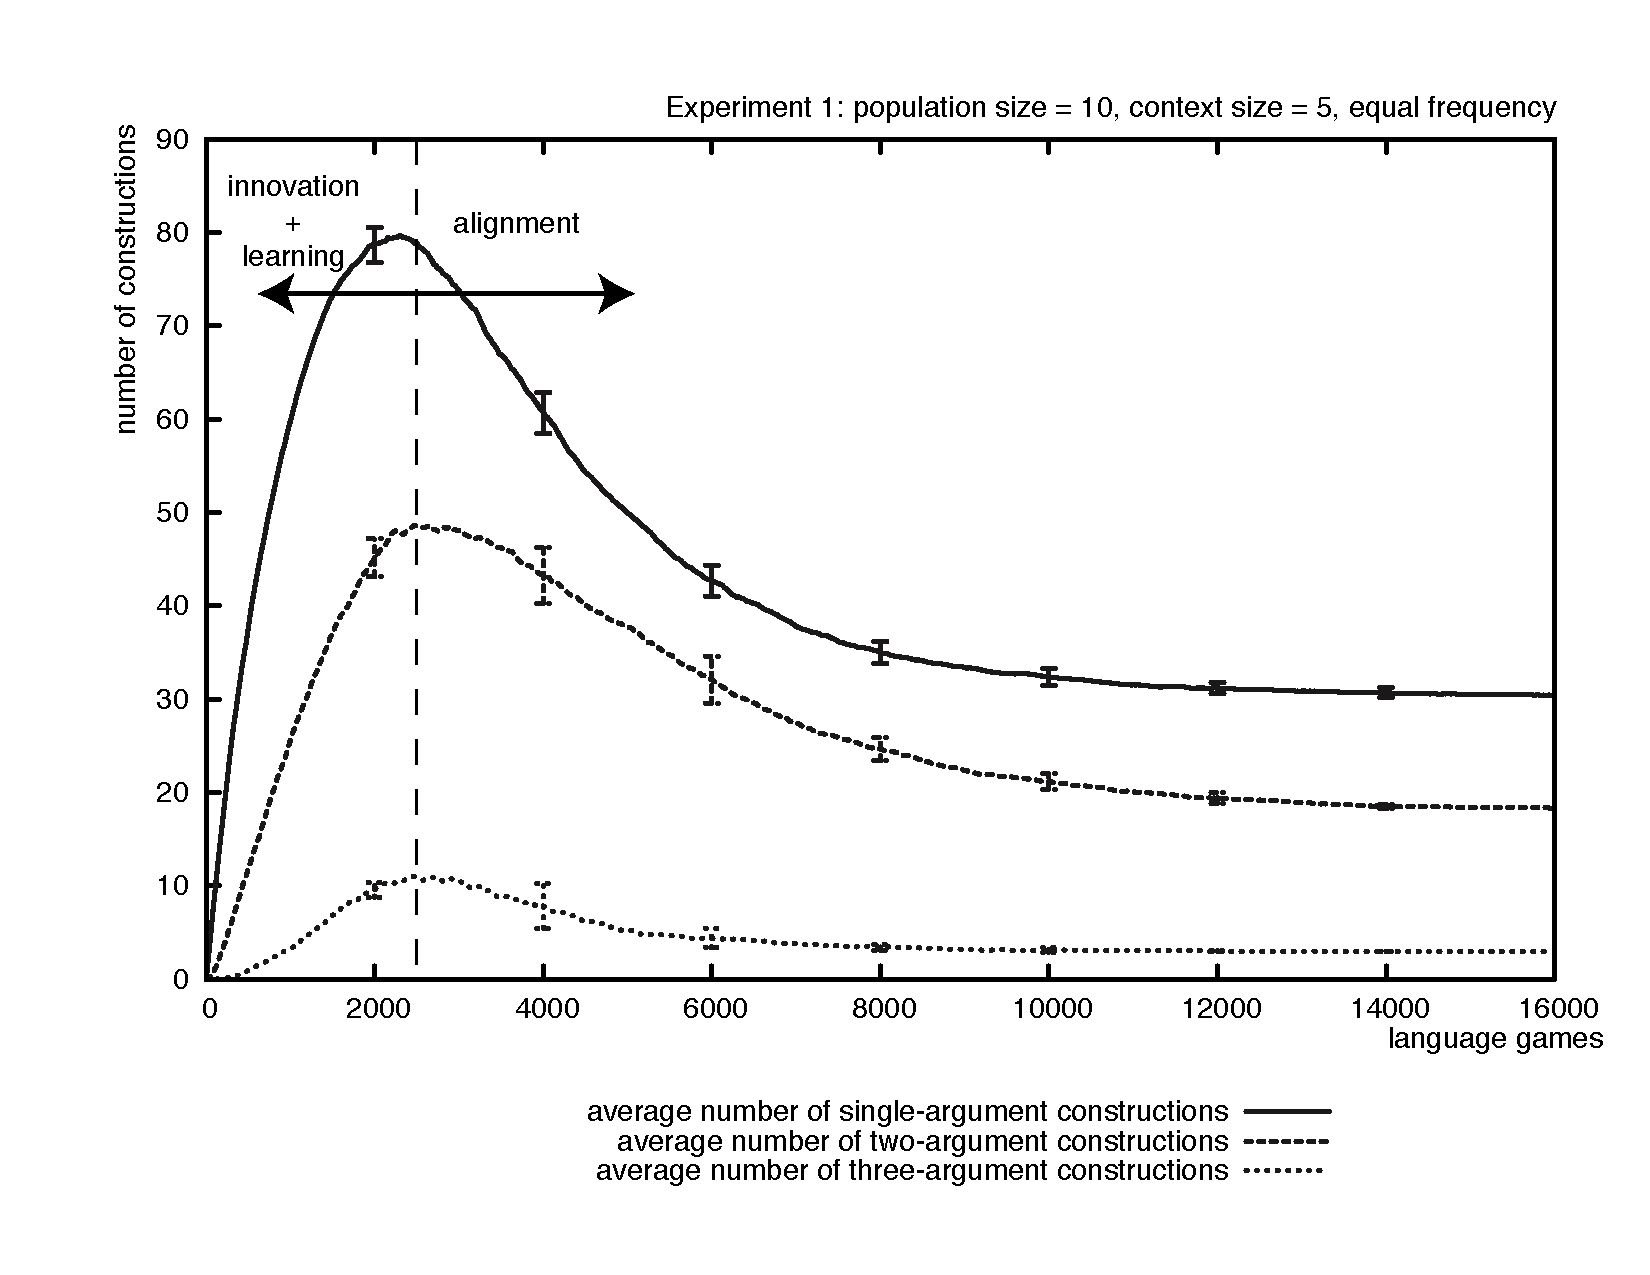
\includegraphics[width=0.85\textwidth]{Chapter4/figs/size2a}}
  \caption[Experiment 1: number of constructions with individual selection]{This graph shows the average number of constructions in a population\is{speech population} of ten agents in experiment 1. In this set-up the agents succeed in converging on an optimal inventory size -- given their cognitive abilities -- of 30 single-argument constructions, 18 two-argument constructions and 3 three-argument constructions. The graph here indicates that there is still an average of 19 two-argument constructions but this competit\is{competition}ion also gets resolved if more language game\is{language game}s are played.}
   \label{f:size1}
\end{figure}
\begin{figure}[htb]
\centerline{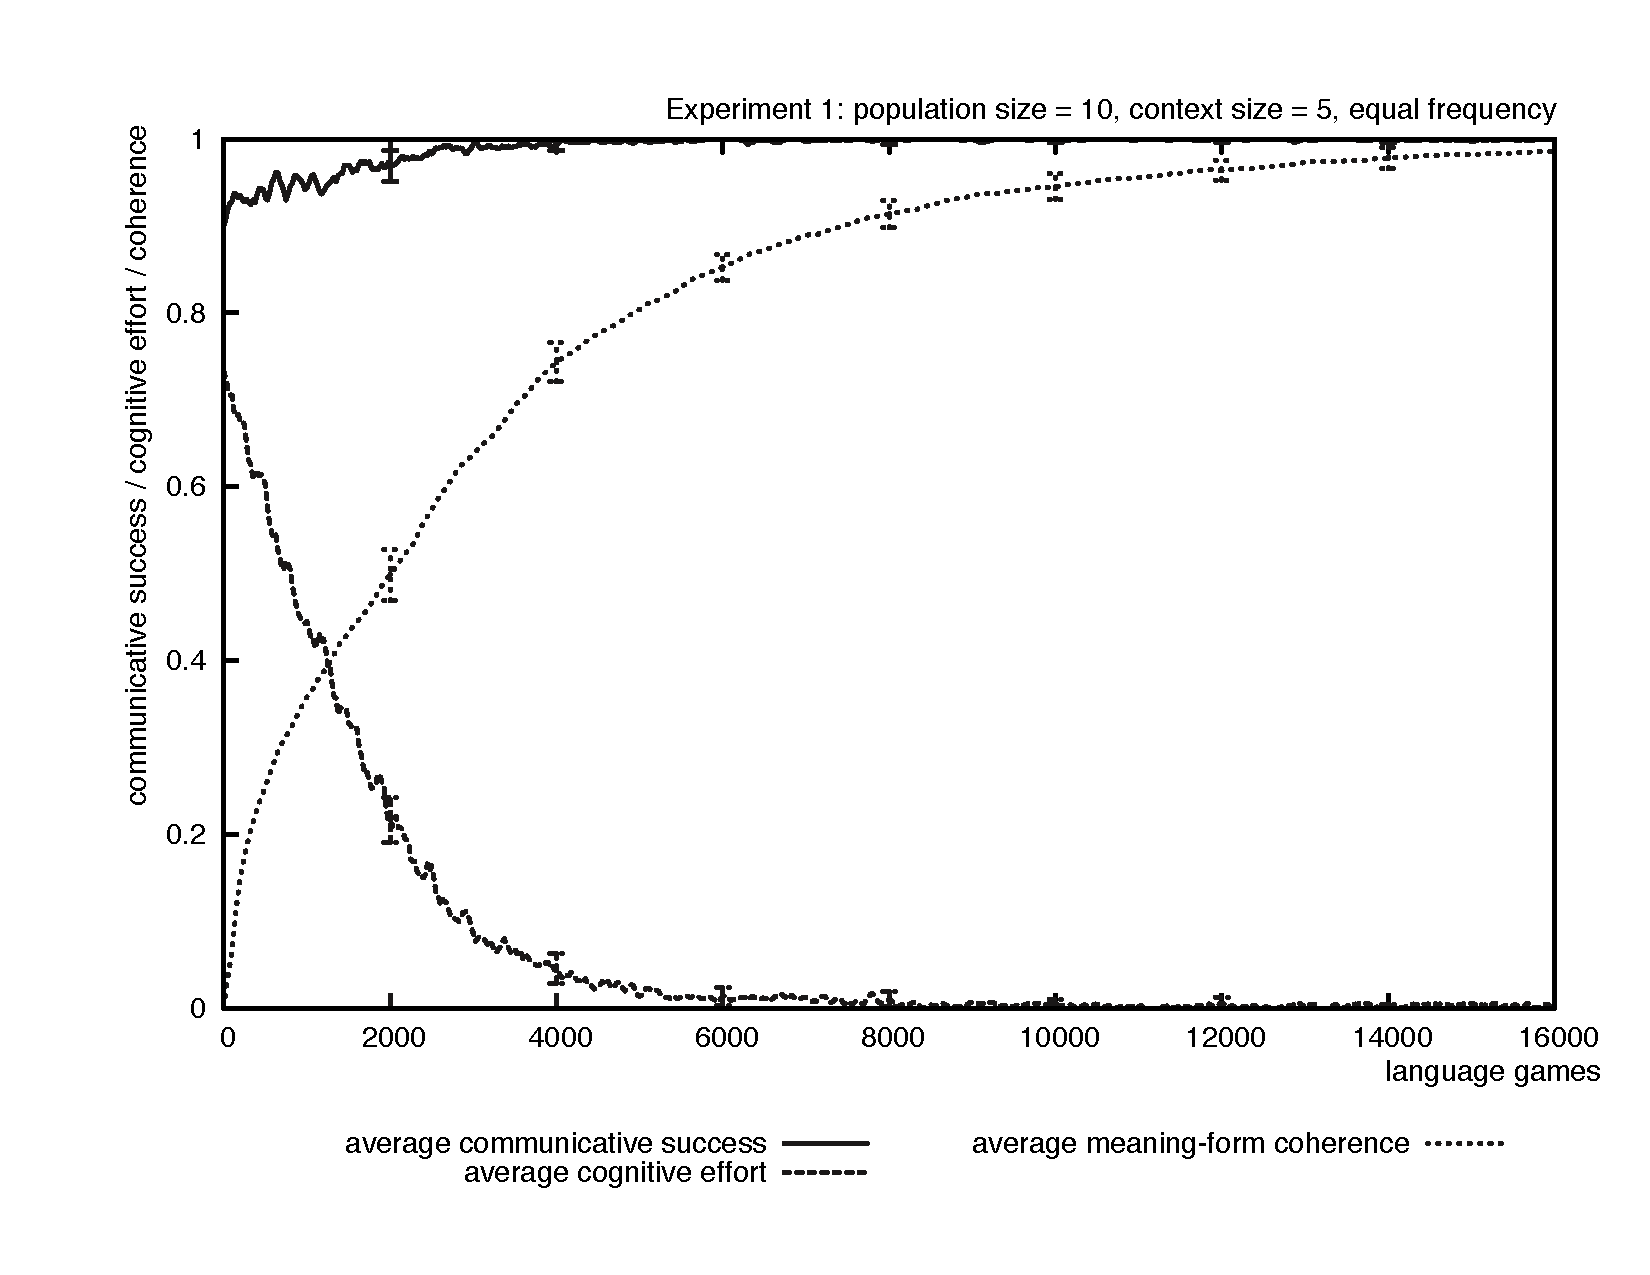
\includegraphics[width=0.85\textwidth]{Chapter4/figs/effort2a}}
  \caption[Experiment 1: success, effort and coherence]{This graph shows average communicative success\is{communicative success}, cognitive effort\is{cognitive effort} and meaning-form coherence in a population\is{speech population} of ten agents in experiment 1. The results show that the agents succeed in reaching 100\% communicative success\is{communicative success} and reducing the cognitive effort\is{cognitive effort} needed for communication. Meaning-form coherence reaches almost 100\% with only competit\is{competition}ion between one or two forms that is still undecided.}
   \label{f:effort1}
\end{figure}

\subsubsection{Results}
 The experimental set-up was tested in ten series of 16.000 language game\is{language game}s. By looking at the same measures as in the baseline experiments, the simulations seem to yield successful results at first sight. Figure \ref{f:size1} plots the average number of constructions in the population\is{speech population}. Here, the agents have almost reached the optimal state in terms of linguistic inventor\is{linguistic inventory}y. Only in the case of two-argument constructions there are additional language game\is{language game}s needed for deciding on the competit\is{competition}ion between one or two surviving constructions. Acquiring the constructions happens quite fast (in less than 3.000 games), but alignment takes much more time than was needed in the baseline experiments. This is due to the individual selection alignment strateg\is{alignment strategy}y: if a pattern was used, only competing patterns are punished through lateral inhibition\is{lateral inhibition}. The individual marker\is{case!case marking}s or rather the single-argument constructions they occur in are not considered during consolidation\is{consolidation}.
\begin{figure}[p]
\centerline{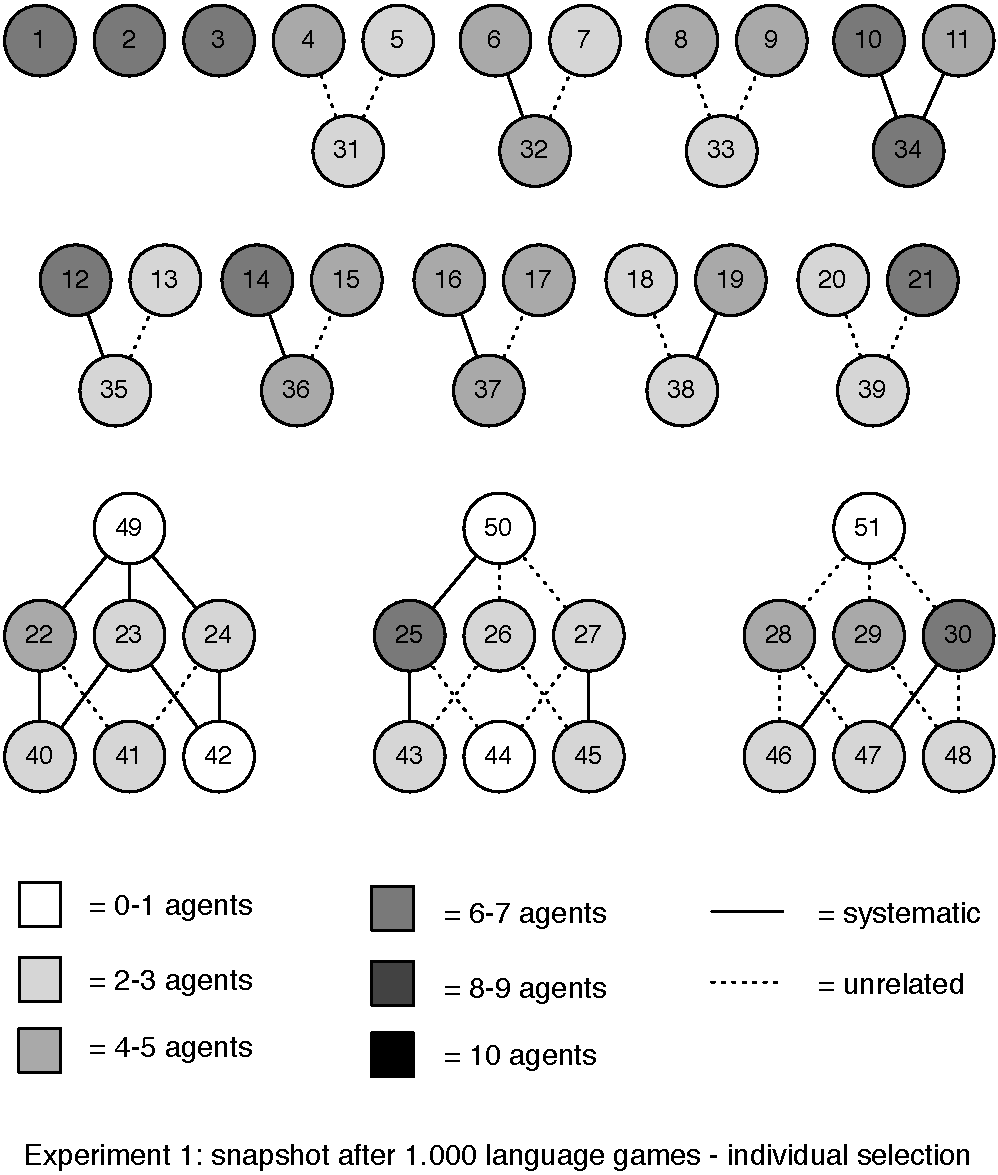
\includegraphics[width=0.7\textwidth]{Chapter4/figs/direct-coherence-no-analogy-1000}}
  \caption[Experiment 1: snapshot after 1.000 games]{This diagram gives a snapshot of the average coherence in a population\is{speech population} of 10 agents after 1.000 language game\is{language game}s using the direct selection alignment strateg\is{alignment strategy}y. Each circle stands for a particular meaning (see the Appendix), for example circles 4 and 5 stand for `appear-1' and `appear-2'. The lines between circles means that the meanings combine into compositional meanings, for example circle 31 means the combination `appear-1 appear-2'. The darker the circle is colour\is{colour}ed, the more agents prefer the same case marker\is{case!case marking}(s) for covering this meaning. A full line between circles means that both meanings are covered using the same marker\is{case!case marking}s (= systematic), a dotted line means that a different form is preferred for the same meaning (= unrelated). The diagram shows that for most meanings only half of the population\is{speech population} prefer the same form and that in many cases there is no systematic choice for a certain case marker\is{case!case marking}.}
   \label{f:1-coherence-1000}
\end{figure}

The long alignment period is also illustrated in Figure \ref{f:effort1}, which displays average communicative success\is{communicative success}, cognitive effort\is{cognitive effort} and meaning-form coherence. The fact that communicative success\is{communicative success} rapidly rises to 100\% within 4.000 language game\is{language game}s and that cognitive effort\is{cognitive effort} drops to zero between 6.000 and 8.000 language game\is{language game}s suggests that the agents have learned all the variation\is{variation}s floating around in their population\is{speech population}. However, meaning-form coherence takes much longer to rise to its maximum which is again due to the alignment strateg\is{alignment strategy}y. Coherence reaches almost 100\% after 16.000 games with only competit\is{competition}ion going on for one or two cases of two-argument constructions. This competit\is{competition}ion will in the end also be resolved after additional language game\is{language game}s.

The longer alignment period is however not the most fundamental problem with the artificial languages that are formed by the agents. A closer examination of them shows that all meaning-form mappings that they agree on are totally arbitrary. The problem is illustrated in Figures \ref{f:1-coherence-1000} and \ref{f:1-coherence-7000} which give a snapshot of convergence and coherence in one simulation after 1.000 and 7.000 language game\is{language game}s respectively. Each meaning or combination of meanings (see the Appendix) is represented as a circle. For example, the meaning `approach-1' is represented as circle 4 and meaning `approach-2' is represented as circle 5. Lines between circles indicate that the meaning of one circle is a combination of the meanings of the other circles. For example, circle 31 combines `approach-1' and `approach-2'. The colour\is{colour} of the circles represents the number of agents that prefer the most frequent form in the population\is{speech population} for that particular word. A white circle means that there is either no form yet for this meaning or that there is no form which is preferred by more than one agent. A black circle means that all ten agents prefer the same form for this meaning. If all the circles are black, the agents have reached 100\% convergence. If the lines between the circles are full lines, the same participant role is expressed by the same marker\is{case!case marking} across constructions. If however the line is dotted, there is a different form for the same meaning.

This can best be illustrated through an example. The circle for meaning 4 (approach-1) indicates that there are 4  or 5 agents in the population\is{speech population} which prefer the same form for marking this participant role at this stage of the simulation. For circles 5 (approach-2) and 31 (approach-1 approach-2), there are two or three agents that prefer the same form. The dotted lines between the circles, however, indicate that the most frequent pattern for circle 31 uses different marker\is{case!case marking}s than the single-argument constructions for circles 4 and 5:

\ea
\gll jack -lich approach\\
jack approach-1 approach\\
\glt `Jack approaches (someone)'.\\

\item
\gll jill -sut approach\\
jill approach-2 approach\\
\glt `(Someone) approaches Jill'.\\

\item
\gll jill -xa jack -zuih approach\\
jill approach-2 jack approach-1 approach\\
\glt `Jack approaches Jill'.\\
\z

\begin{figure}[p]
\centerline{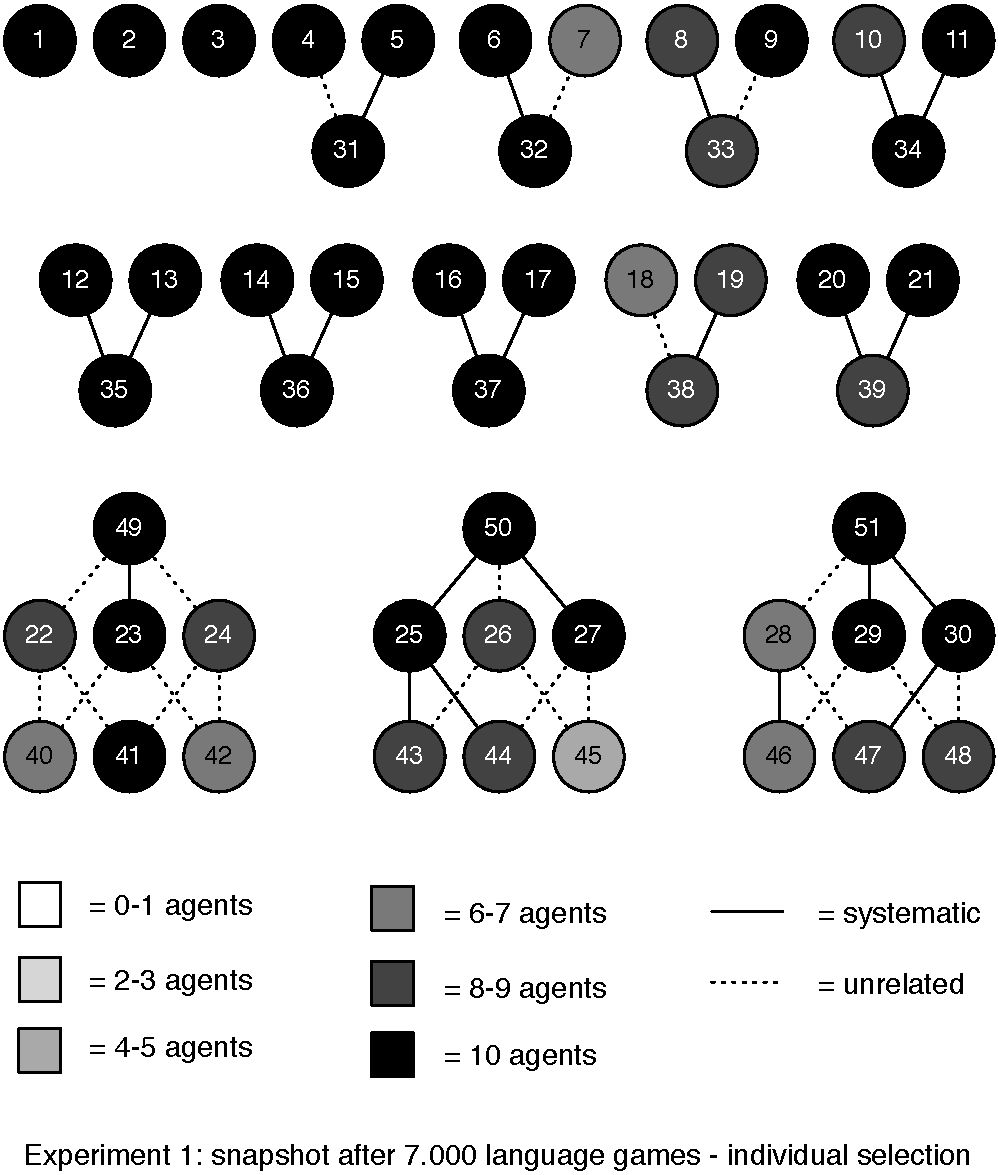
\includegraphics[width=0.7\textwidth]{Chapter4/figs/direct-coherence-no-analogy-7000}}
  \caption[Experiment 1: snapshot after 7.000 games]{This diagram gives a snapshot of the average coherence in a population\is{speech population} of 10 agents after 7.000 language game\is{language game}s using the direct selection alignment strateg\is{alignment strategy}y. The agents have reached convergence for most meanings by now, but these form-meaning mappings are not always systematically related to each other. For example, the meanings related to 49 were pretty consistent in their meaning-form mappings after 1.000 games, but have now become totally unrelated to each other: for each possible combination a new form is introduced to cover the same meaning. In all the cases where there is no systematicity\is{systematicity}, the convergence is not complete yet.}
   \label{f:1-coherence-7000}
\end{figure}

Figure \ref{f:1-coherence-7000} shows that after 7.000 language game\is{language game}s, the agents have almost converged on a form for every meaning, but the problem of systematicity\is{systematicity} remains: in half of the cases, a different case marker\is{case!case marking} is winning the competit\is{competition}ion on the level of single-argument constructions than the one(s) winning on the other levels. The figure also shows that in most of the cases where there is no systematic use of a form for the same meaning, convergence is also still not complete. This is in contrast to the meanings which (accidentally) arrived at the same form across constructions. Here we see mostly black circles meaning that all agents prefer the same convention\is{convention}.


\subsubsection{Discussion}
 The results clearly indicate that the agents are not capable of constructing a systematic language. The reason for this is that all constructions are basically treated as independent linguistic items. This means that once a larger pattern is created, it starts living its own life without influencing or being influenced by the constructions that were used to create it. This results in some case marker\is{case!case marking}s losing the competit\is{competition}ion for marking a certain participant role on the level of single-argument constructions but still becoming the most successful one as part of a larger pattern. In all the simulations, this happened in 40 to 60\% of the cases (see Figure \ref{f:systematicity2}).

The fact that in more than half of the cases the same marker\is{case!case marking} wins the competit\is{competition}ion on all levels is due to the small meaning space of the experiment and the fact that patterns are always created by combining the most successful constructions at a given point in the simulation. In fact, the agents can continue to create new patterns for a certain combination of participant roles even if they already know other patterns for it. For example, it may happen that on a lower level the average confidence\is{confidence} scores of a new combination becomes more successful than the confidence\is{confidence} score of the patterns. In this case the agents will still innovat\is{innovation}e which gives a slight advantage to those patterns that are in line with the most successful constructions of a lower level. As the results show, however, this is not enough.

Since natural languages are also not fully regular, it is important to see whether the lack of systematicity\is{systematicity} in the experiments is relevant for the many exceptions and sub-regularities found in natural languages. The answer is no: for most if not all irregular forms and sub-regularities in natural language, either a systematic origin can be found through diachron\is{diachronic}ic changes or through external pressures such as language contact\is{language contact}. For example, the -ed-participle in English\is{English} did not manage to exten\is{extension}d its use to all past tense\is{tense}s as can be observed in irregular verb\is{verb}s such as {\em to sing} and {\em to give}. These strong verb\is{verb}s are however remnants of completely regular classes of verb\is{verb}s in Proto-Indo-European that were able to survive thanks to their high token frequency\is{token frequency}\is{frequency}. Despite all sociological factors, historical incidents, language contact\is{language contact}, and other kinds of exceptions, natural languages succeed remarkably well in developing systematicity\is{systematicity} spanning over many constructions, as for example word order in English\is{English}. Given the abstraction\is{abstraction}s and scaffold\is{scaffold}s of the present experiments, the agents should thus be capable of developing a fully systematic language without any problems.

This leaves us the question of how systematicity\is{systematicity} can be achieved. As said before, all systematic form-meaning mappings have been formed by accident due to the small world and the nature of the innovat\is{innovation}ion mechanism. For true systematicity\is{systematicity}, however, the agents need to be able to recognize relations between constructions rather than treating them as a list of independent units. This would mean that if a particular construction is successful, its systematically related constructions should also (perhaps indirectly) benefit from its success. In section \ref{s:pattern-exp-2} I will introduce a biologically inspired mechanism that can be exploited to achieve this effect: multi-level selection\is{multi-level selection}.

\subsection{The problem of systematicity\is{systematicity} in other work}
\label{s:problem-systematicity}

As to my knowledge, the problem of systematicity\is{systematicity} has never been reported before in the field of the origins\is{origins} and evolution\is{evolution!cultural evolution} of language. This does not mean, however, that the problem never existed. In this section, I will give a brief overview of some prior work in the field in which the problem was either overlooked or in which it could not occur due to experimental assumption\is{assumption}s.


\subsubsection{Exemplar-based\is{exemplar-based models} simulations}
 One computational simulation which is closely related to the work in this book is presented by \citet{batali02negotiation}. Batali investigates how a multi-agent population\is{speech population} can form a recursi\is{recursion}ve communication system by using exemplars stored in memory. This work can be categorized as a `problem-solving\is{problem-solving} model' because these exemplars have to be agreed upon in locally situated interactions. Each exemplar has a confidence\is{confidence} score which is increased and decreased according to similar lateral inhibition\is{lateral inhibition} dynamics as in the simulations of the previous section. The type of learner is thus the same one as the agents in this book: they build their language instance by instance in a bottom-up and redundant fashion. Batali's agents only keep exemplars and all generalization in the model is captured by directly manipulating these exemplars during processing. Figure \ref{f:batali} gives an example of an exemplar composed of two smaller ones \citep[exemplar 5.1.2.a]{batali02negotiation}.
\begin{figure}[h]
\centerline{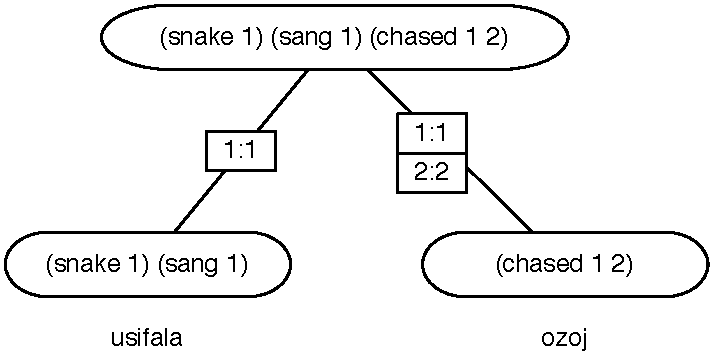
\includegraphics[width=0.75\textwidth]{Chapter4/figs/batali}}
  \caption[An exemplar \citep{batali02negotiation}]{A complex exemplar from \citet{batali02negotiation}. The exemplar features a compositional meaning with `argument maps' to the smaller exemplars that take care of variable equal\is{variable equality}ities in the meaning.}
   \label{f:batali}
\end{figure}

Batali does not use event-specific variables as I do in this book but assumes a simple three-way contrast between arguments 1, 2 and 3. For example the meaning ((snake 1) (sang 1)) translates to something like `the snake sang', whereas ((snake 1) (sang 2)) would mean something like `there was a snake and something sang.' Event structure\is{event structure} is stored immediately in the exemplar but can be overridden by argument maps between complex exemplars and their subcomponents. For example, the argument map `1:2' translates a meaning like (rat 1) to (rat 2). These argument maps are also stored as part of the complex exemplar. Apart from these argument maps between complex exemplars and their components, all exemplars are unrelated and listed in the memory.

The agents then engage in a series of description game\is{language game!description game}s. They are able to invent new words for new meanings and they are capable of combining existing words into larger patterns or breaking up a pattern again into smaller parts. The ultimate goal of the agents is two-fold: (a) agree on a shared lexicon\is{lexicon} for all the single meanings (e.g. cat, fox, chase, etc.) and (b) agree on a way to mark event structure\is{event structure} through the argument maps (i.e. marking the difference between arguments 1, 2 and 3). The simulations make use of a single generation of agents.

The results indicate that the agents gradually reach communicative success\is{communicative success} and that they agree on the same exemplars. Goal (a) is therefore definitely reached. However, the results show that event structure\is{event structure} is not always marked in the same way: all the simulations end up using specific ordering for each exemplar (even though they may involve the same meanings) and using `empty' words that accidentally evolved into marker\is{case!case marking}s for argument mappings. The agents thus do not succeed in agreeing on a systematic way of distinguishing participant `1' from participants `2' and `3'. The agents thus cannot generaliz\is{generalization}e argument mapping to new predicates such as (give 1 2 3) and have to negotiat\is{negotiation}e event structure\is{event structure} for each word separately. This lack of systematicity\is{systematicity} is not noted by Batali as a problem and the use of the empty words is wrongly interpreted as corresponding to argument marker\is{case!case marking}s in natural languages.


\subsubsection{Probabilistic grammars}
 Another experiment in which the systematicity\is{systematicity} problem is overlooked is reported by \citet[chapter 10]{depauw02grael}. De Pauw investigates how rudimentary principles of syntax can emerge from distributional aspects of communication rather than from the interface\is{syntax-semantics interface} between syntax and semantics. This exclusive focus on syntax is different from the work in this book (even though some semantics is smuggled into De Pauw's simulations in the disctinction between animate\is{animacy} and non-animate\is{animacy} objects which results in different distributional patterns). Similar assumption\is{assumption}s to this book are the heavy use of memory (even more so by De Pauw), a bottom-up and redundant formation\is{formation} of the language and a predefined lexicon\is{lexicon} in order to focus exclusively on the topic of interest. The population\is{speech population} in De Pauw's simulations is dynamic in the sense that there is a generational turn-over, but no linguistic information is transmitted genetically from one generation to the next.

The agents engage in a series of language game\is{language game}s in which they communicate about objects or events. If there are several objects, the agents can choose between six word orders: SVO, SOV, VSO, VOS, OSV or OVS. De Pauw therefore does not distinguish between verb\is{verb}-specific participant roles, but only assumes a two-way contrast between the subject\is{syntactic role!subject} (S) and the object\is{syntactic role!object} (O). The agents start without any preference for a particular word order so variation\is{variation} naturally occurs in the population\is{speech population}. The alignment strateg\is{alignment strategy}y of the agents is simply storing bigrams or frequencies of co-occur\is{co-occurrence}rences and performing statistical inducti\is{induction}on on top of those bigrams \citep[362]{depauw02grael}:

\begin{figure}[h]
\centerline{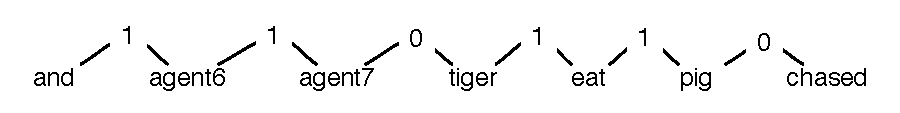
\includegraphics[width=\textwidth]{Chapter4/figs/depauw}}
  \caption[Bigram probabilities \citep{depauw02grael}]{The agents in \citet{depauw02grael} store co-occur\is{co-occurrence}rence frequencies and use these bigram-probabilities to decide on a preferred ordering.}
   \label{f:depauw}
\end{figure}

During the simulations, the agents rapidly converge on fixed word order on simple relations. However, as De Pauw notes, there are no general tendencies in terms of a general word order. Each `verb' rather has its own preferred ordering. For more complex relations, the agents do not always reach coherence. De Pauw concludes that the agents therefore reside in a local maximum and that they evolve from one local maximum of convergence to the next. De Pauw argues that this is not a shortcoming of the model but rather its greatest asset: whereas other models in the field are looking for the state of convergence, {\em ``language itself never converges and constantly adapts to a changing environment and seems to be driven by chaotic elements, introducing a large degree of randomness in language both from a synchron\is{synchronic}ic, as well as a diachron\is{diachronic}ic point of view''} (p. 378).

There are however no such chaotic elements present in De Pauw's model which should prevent the agents from reaching complete coherence. The degree of randomness in his simulations seems to stem from the systematicity\is{systematicity} problem: by only looking at bigram probabilities, it is to be expected that there is an arbitrary word order which is verb\is{verb}-specific. In the case of more complex predicates, the preferred order depends on a combination of various bigrams which increases the randomness because the probabilities of these bigrams are constantly changing so it becomes much harder to agree on a fixed order for these complex meanings. De Pauw dismisses the possibility that the degree of convergence is the maximum that can be expected from the population\is{speech population}, but this is in fact the only correct conclusion. Given the cognitive capabilities of the agents, convergence could only increase if the input would be more structured. In certain machine learning\is{machine learning} tasks, there is already a lot of structure present in the learning data so bigrams can be successfully used for making some predictions. In the case of language formation\is{formation}, however, agents have to start from scratch so there is no structure spanning multiple levels yet that can be induced.

De Pauw's concluding remark is that it is empirically impossible to know whether the agents succeed in {\em ``expressing the proper (agent, patient) relationship, or if it is just a side-effect of beneficial bigram probability distributions''} (p. 376). I would argue, however, that since the agents are not endowed with the capacity of relating bigrams to each other but solely rely on these probabilities, all tendencies in word order are in fact a side-effect of the bigrams. The conclusion is that \citet{depauw02grael}, just like \citet{batali02negotiation}, misinterpreted experimental results because the problem of systematicity\is{systematicity} was not noticed.


\subsubsection{Iterated Learning Model\is{Iterated Learning Model (ILM)}s}
 So far I only discussed models that featured lazy learner\is{lazy learner}s: agents which postpone generalization until processing time and which shape their language in a step-by-step fashion. As opposed to lazy learner\is{lazy learner}s there are `eager learner\is{eager learner}s'. Eager learner\is{eager learner}s try to look for generalizations (and abstraction\is{abstraction}s) before it is actually needed in processing and work on the complete inventory. Eager learner\is{eager learner}s typically discard the examples that can be deriv\is{derivation}ed from a rule and thus try to optimize the inventory size. If the problem of systematicity\is{systematicity} also occurs with eager learner\is{eager learner}s, then we know that the problem is not exclusive to the usage-based approach\is{usage-based model} proposed in this book. 

In the field of artificial language evolution\is{artificial language evolution}, especially Iterated Learning Model\is{Iterated Learning Model (ILM)}s feature agents that loop through their inventory after each interaction in order to make abstraction\is{abstraction}s. In section \ref{s:impact} I will draw a thorough comparison between my experimental results and those of \citet{moy06case}, who investigated the same topic using the Iterated Learning Model\is{Iterated Learning Model (ILM)} so I will not go into details here. As a quick preview, I can already give away one of the conclusions which is that the problem of systematicity\is{systematicity} also occurs in Iterated Learning Model\is{Iterated Learning Model (ILM)}s. This does not only happen in Moy's experiments, but also in the simulations reported by \citet{kirby00syntax} and \citet{smith03iterated} even though these models feature complete meaning transfer and a population\is{speech population} of only two agents.

The conclusion is the same as for the other simulations reported in this section: the problem of systematicity\is{systematicity} goes by unnoticed in most Iterated Learning Model\is{Iterated Learning Model (ILM)}s, but becomes very apparent in \citet{moy06case}. The problem occurs for the same reasons as in all the other experiments: the agents only behave `systematic' during innovat\is{innovation}ion and learning, but then treat all linguistic items as an unstructured list of unrelated elements. So either there is no adequate model yet that avoids the problem of systematicity\is{systematicity} or the problem is {\bfseries not restricted to the type of learner}. In the latter case, the problem seems to be caused by the fact that the linguistic inventor\is{linguistic inventory}y is unstructured.


\subsubsection{Other models}
 Finally, there are many models that investigate certain aspects of grammar in which the problem of systematicity\is{systematicity} does not occur such as \citet{debeule07compositionality, debeule06emergence, nowak99evolution, steels06how-grammar}; etc. I will take the simulations by \citet{debeule06emergence} as an example of why these models don't have the problem. The conclusions of this brief discussion extend to all the other models on grammar as well.

De Beule \& Bergen investigate the competit\is{competition}ion between holistic and compositional utterances. In case of compositional utterances, one could expect the problem of systematicity\is{systematicity} to pop up, but it doesn't. The reason is that De Beule \& Bergen designed their experiment in such a way that the agents had prior knowledge about what kind of categories and constructions to expect: individual words are immediately tagged with a certain syntactic category and grammatical constructions are fully schematic from the start. One construction can hence be used for all possible combinations of competing individual words that are tagged with the same category and remains agnostic as to which words should win the competit\is{competition}ion. The experiment thus made a clear separation between the lexicon\is{lexicon} on the one hand and grammatical constructions on the other; and it did not offer the agents the possibility of in-between patterns or idiom\is{idiom}s.

This is not a criticism of the model per se: given the fact that De Beule \& Bergen only intended to focus on competit\is{competition}ion between holistic and compositional utterances, the design choice is justified in which the competit\is{competition}ion dynamics can be clearly investigated on each level. As such the experiment can be interpreted as investigating a prerequisite of grammar rather than the emergence\is{formation} of {\em actual} grammar. For the scope of this book, this experimental design is thus not warranted: the barrier between fully idiom\is{idiom}atic items and fully schematic items needs to be broken down.

\section{Experiment 2: multi-level selection\is{multi-level selection} without analog\is{analogy}y}
\label{s:pattern-exp-2}

In the previous section I demonstrated the problem of systematicity\is{systematicity} that occurs during the emergence\is{formation} of a language if the agents treat all entries in their linguistic inventor\is{linguistic inventory}y as unrelated individuals and if their language comprises multiple layers of organization. An alignment strateg\is{alignment strategy}y involving the individual selection of constructions leads to completely arbitrary form-meaning pairs whereas natural languages show greater cohesion and a higher degree of systematically related constructions. Even in idiom\is{idiom}s such as {\em he kicked the bucket}, some degree of schematicity is present such as the conjugation of the verb\is{verb}. The agents therefore need a new alignment strateg\is{alignment strategy}y in which the success of one construction may have an impact on the success of other related constructions.

In this section I will present an experiment which features new alignment strateg\is{alignment strategy}ies that are inspired by the notion of `multi-level selection\is{multi-level selection}' in evolutionary biology \citep{wilson94group}. Multi-level selection\is{multi-level selection} (formerly known as `group selection') acknowledges the fact that groups or other higher-level entities can act as `vehicles' for selection. In this view, not all aspects of groups are reduced to by-products of individual (and usually selfish) interactions. In other words, being part of a group can increase the selectionist advantage of individuals.% One example from biology concerns the origins of chromosomes. Individual genes started to be combined into larger units (chromosomes). The genes are on the one hand replicators in their own right, undergoing competit\is{competition}ion, but they are also part of the larger replicating unit of chromosomes \citep{maynard-smith93origin}.

Natural languages are clear instances of organisms with a hierarchical functional organization which can be conceived as `groups within groups'. Competition is going on at multiple levels of this organization: between synonyms for becoming dominant in expressing a particular meaning, between idiom\is{idiom}atic patterns that group a number of words, between different syntactic and semantic categories competing for a role in the grammar, between ways in which a syntactic category is marked, etc. Multi-level selection\is{multi-level selection}s therefore seems to be readily applicable to language as well.

\subsection{Experimental set-up}

The most important requirement for implementing multi-level selection\is{multi-level selection} is that the agents have to be capable themselves of recognizing relations between linguistic items. This is in fact not so difficult to achieve: in section \ref{s:operationalizing-patterns} I explained that the agents keep a link between larger constructions and the constructions that were used for creating them. These links can now be used for implementing multi-level selection\is{multi-level selection}. Three different alignment strateg\is{alignment strategy}ies have been implemented for comparison:

\begin{itemize}
\item {\bfseries Top-down selection}: if the game was a success, the hearer will not only reward the constructions that were applied during processing, but also all the related constructions on a lower level. The confidence\is{confidence} scores of all the competit\is{competition}ors of these constructions are decreased through lateral inhibition\is{lateral inhibition}.
\item {\bfseries Bottom-up selection}: If the game was a success, the hearer will not only increase the score of the applied constructions, but also the scores of all the related constructions on a higher level. All the competing constructions are punished.
\item {\bfseries Multi-level selection\is{multi-level selection}}: If the game was a success, the hearer will not only increase the score of the applied constructions, but also the scores of all related constructions. All the competing constructions are punished through lateral inhibition\is{lateral inhibition}.
\end{itemize}

Retrieving related constructions is performed recursi\is{recursion}vely. For example, if a three-argument construction was applied using the top-down selection alignment strateg\is{alignment strategy}y, its two sub-components are retrieved (a two-argument and a single-argument construction) as well as the two sub-components of the two-argument construction. The hearer thus increases the scores of five constructions. The competit\is{competition}ors are all the direct competit\is{competition}ors of these five constructions.
\begin{figure}[p]
\centerline{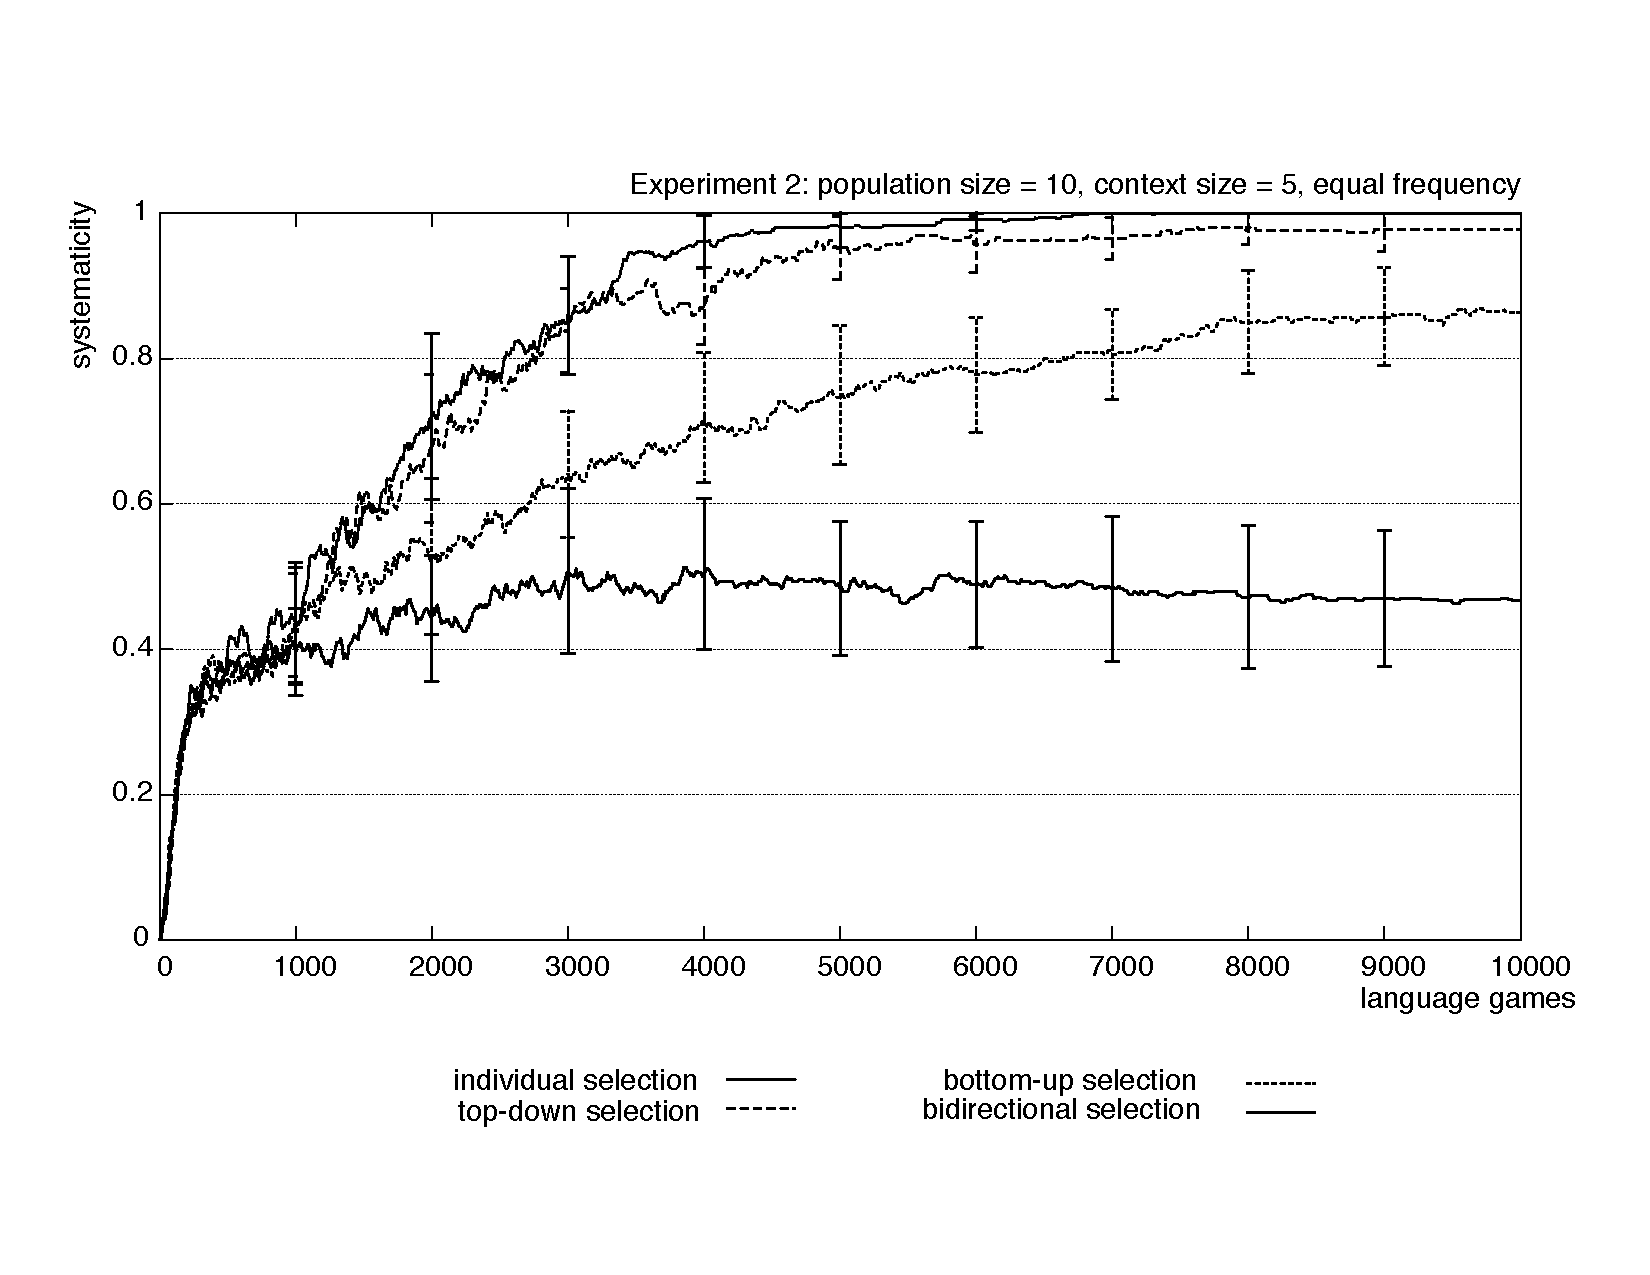
\includegraphics[width=\textwidth]{Chapter4/figs/systematicity-vs-2}}
  \caption[Experiment 2: systematicity]{This graph compares the performance\is{performance} in terms of systematicity\is{systematicity} of four experimental set-ups. systematicity\is{systematicity} fluctuates around 50\% in the baseline case where there is only individual selection (experiment 1). With the bottom-up selection strategy the agents improve the systematicity\is{systematicity} rate to 80\% but then get stuck. Top-down selection leads to full systematicity\is{systematicity} in some of the runs, but most of the simulations feature some `frozen accidents' as well. Only the multi-level selection\is{multi-level selection} strategy leads to full systematicity\is{systematicity} in all the series after about 7.000 language game\is{language game}s.}
   \label{f:systematicity2}
\end{figure}

During processing, only the scores of the applied constructions are taken into account and not of the whole group of related constructions. The group selection dynamics therefore only matter during consolidation\is{consolidation}. The rest of the set-up is the same as for experiment 1.

\subsection{Results and discussion}

\begin{figure}[p]
\centerline{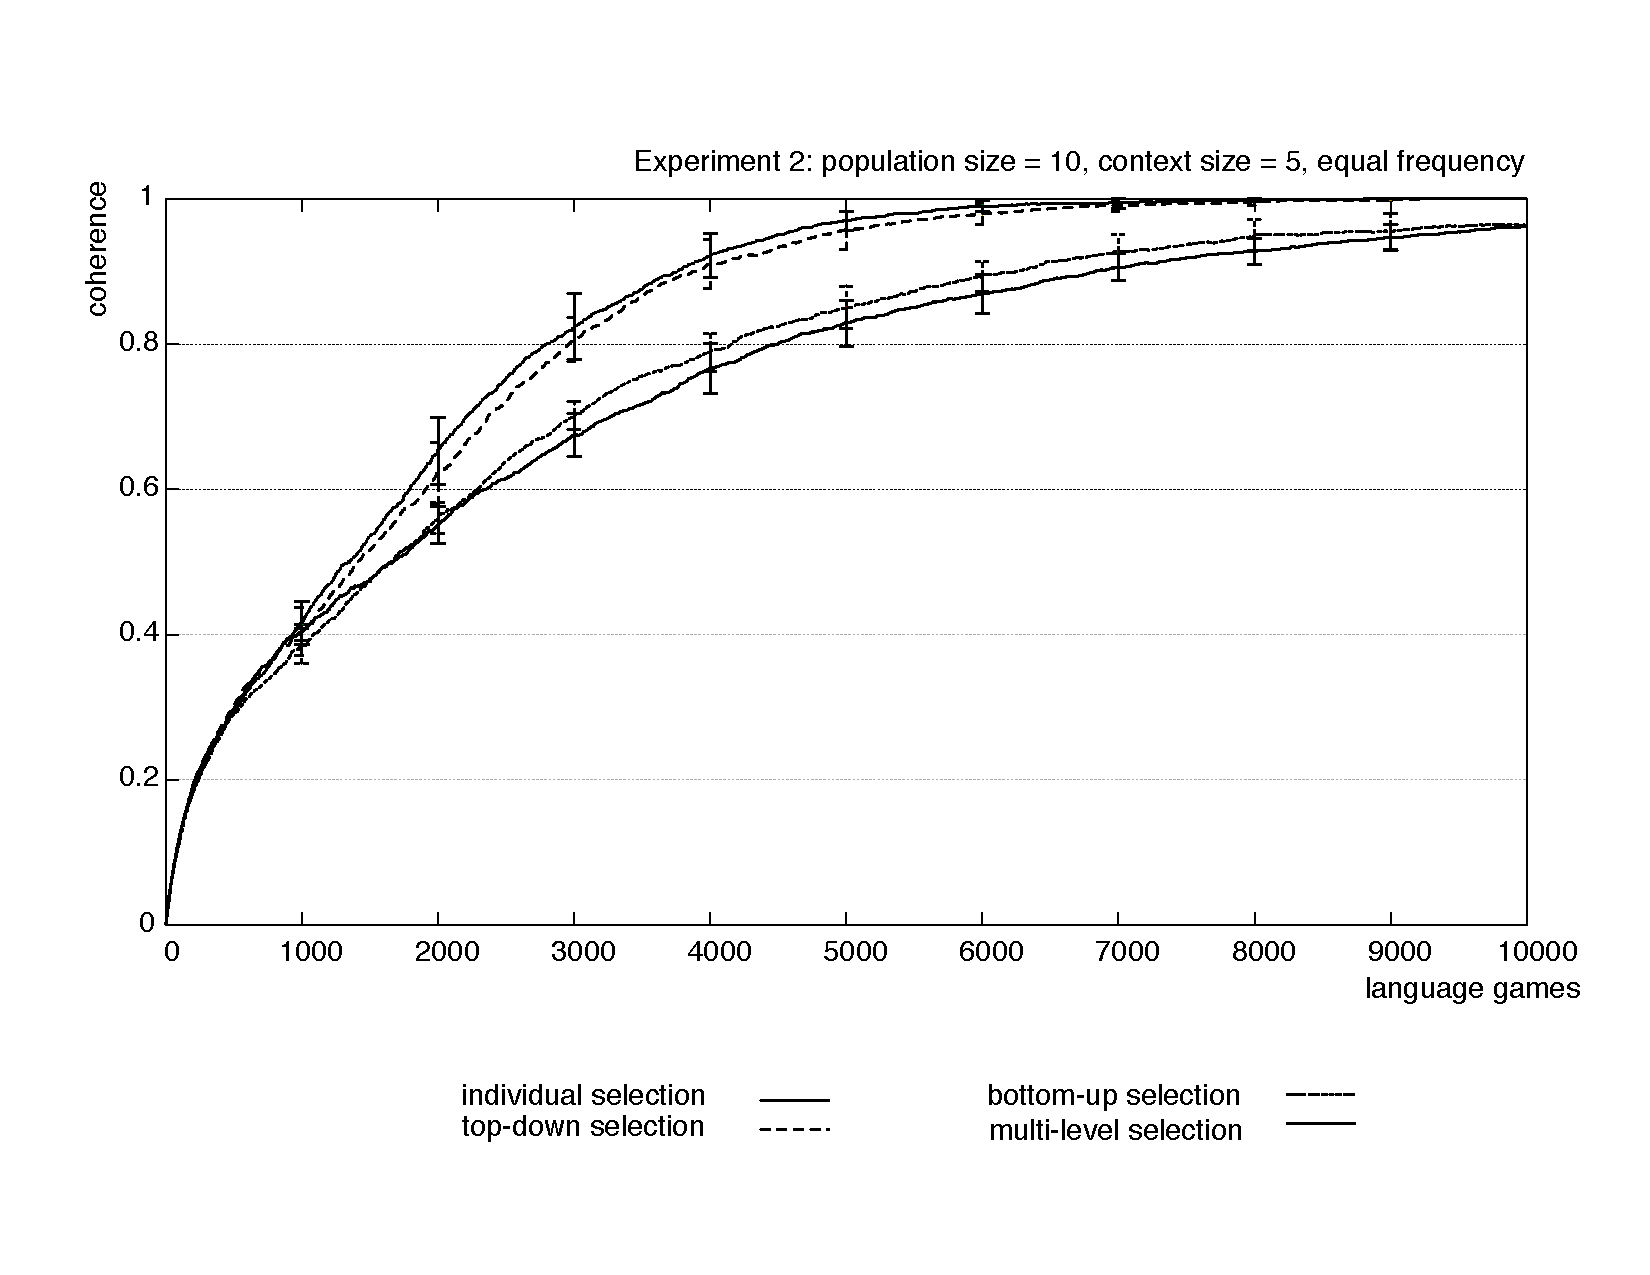
\includegraphics[width=\textwidth]{Chapter4/figs/coherence-vs-2}}
  \caption[Experiment 2: meaning-form coherence]{Since the systematicity\is{systematicity} graph only takes the most frequent forms into account, meaning-form coherence has to be checked in order to verify whether all the agents have converged on the same form-meaning pairs. We see that after 10.000 language game\is{language game}s, only the top-down and the multi-level selection\is{multi-level selection} alignment strateg\is{alignment strategy}ies have already reached complete coherence. Multi-level selection\is{multi-level selection} slightly outperforms top-down selection but not significantly so. In the case of bottom-up and individual selection, the agents need additional language game\is{language game}s for reaching coherence.}
   \label{f:coherence2}
\end{figure}

The three alignment strateg\is{alignment strategy}ies were compared to each other and to experiment 1 in ten series of 10.000 language game\is{language game}s.


\subsubsection{Results}
 Figure \ref{f:systematicity2} illustrates the amount of systematicity\is{systematicity} in all four alignment strateg\is{alignment strategy}ies. The graph shows that the three alignment strateg\is{alignment strategy}ies involving multiple levels all improve on the baseline of individual selection of experiment 1. With the alignment strateg\is{alignment strategy}y of individual selection, systematicity\is{systematicity} fluctuates between 40 and 60\% depending on how `lucky' the agents were. The behaviour of the other three strategies is much more consistent over the ten series. The graph shows that bottom-up selection allows the agents to improve systematicity\is{systematicity} to 80\% but there they are faced with `frozen accidents' as well. The top-down selection improves systematicity\is{systematicity} even further and allows the agents to reach full systematicity\is{systematicity} in some of the runs. However, in most cases, there were still two or three unsystematic patterns left. Only the multi-level selection\is{multi-level selection} strategy led to full systematicity\is{systematicity} in all the simulations.

Since the measure of systematicity\is{systematicity} only looks at the most frequent forms floating in a population\is{speech population}, it needs to be complemented with meaning-form coherence to verify whether {\em all} the agents converge on the same preferences. Figure \ref{f:coherence2} therefore compares the performance\is{performance} of the four alignment strateg\is{alignment strategy}ies in terms of coherence. From the results of experiment 1 we already knew that in the case of individual selection, alignment takes longer than 10.000 language game\is{language game}s. The coherence line for bottom-up selection runs almost parallel with it and does not improve on it in terms of convergence speed. The only two strategies that reach convergence within 10.000 games are top-down and multi-level selection\is{multi-level selection}. Full coherence in the case of top-down selection however does not mean full systematicity\is{systematicity}, as was shown in Figure \ref{f:systematicity2}.

\begin{figure}[t]
\centerline{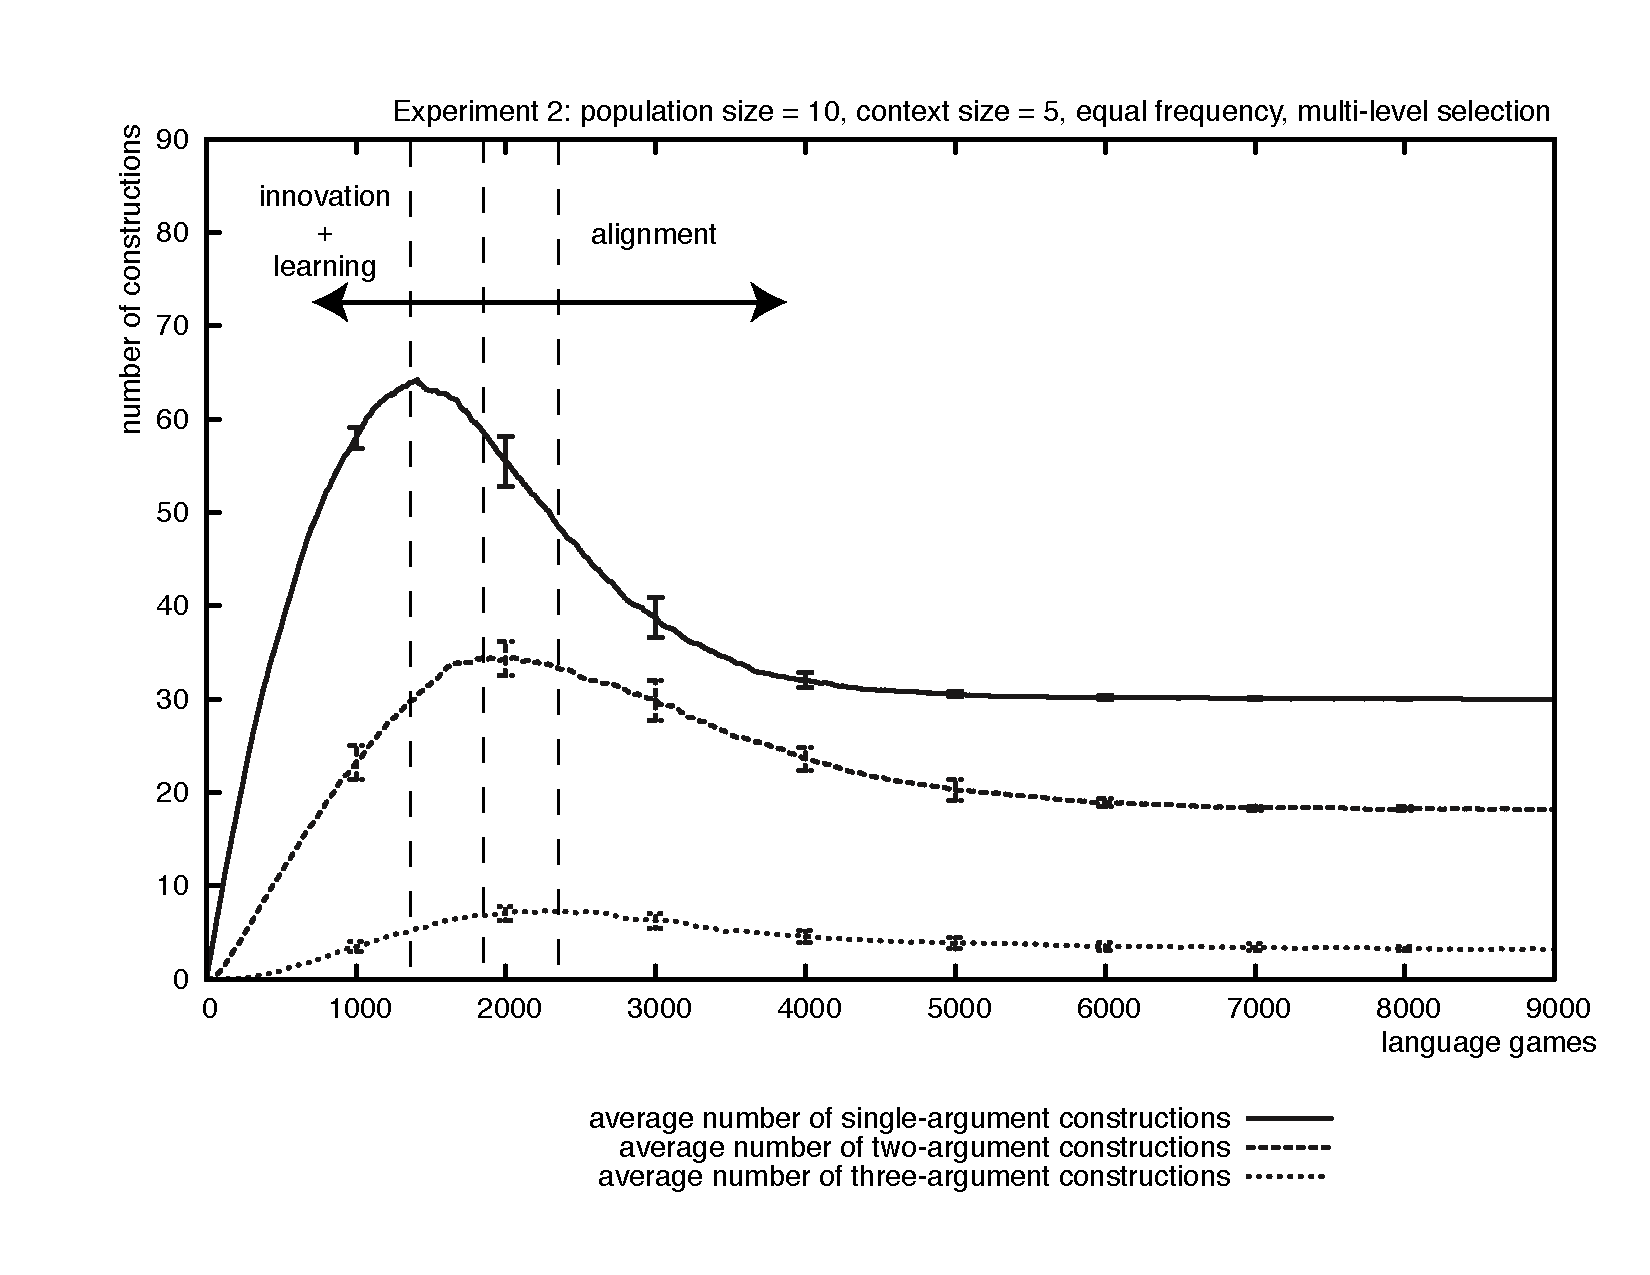
\includegraphics[width=0.87\textwidth]{Chapter4/figs/size2d}}
  \caption[Experiment 2: number of constructions with multi-level selection\is{multi-level selection}]{This graph shows the average number of constructions known by an agent using the multi-level selection\is{multi-level selection} alignment strateg\is{alignment strategy}y. Compared to individual selection, multi-level selection\is{multi-level selection} allows the agents to discard competit\is{competition}ors much more rapidly: there are significantly less variation\is{variation}s floating around in the population\is{speech population}. For example, the peak of single-argument constructions is about 60 instead of 80 in experiment 1. Also the alignment phase happens much faster.}
   \label{f:size2d}
\end{figure}

Figure \ref{f:size2d} shows the average number of constructions in the ten series involving the alignment strateg\is{alignment strategy}y of multi-level selection\is{multi-level selection}. The graph confirms the fact that the agents converge significantly faster on an optimal number of constructions than in experiment 1. At the peak of competing constructions, there are about 60 single-argument constructions, 30 two-argument constructions and 6 three-argument constructions or an average of two competing constructions for each possible meaning. This is much less than in experiment 1 (see Figure \ref{f:size1}) which featured peaks of 80 single-argument, 50 two-argument and 10 three-argument constructions. Also alignment happens much faster: with multi-level selection\is{multi-level selection}, the agents align after 6.000 games as opposed to 14.000 language game\is{language game}s or more if the agents use individual selection.

Figures \ref{f:2d-coherence-1000} and \ref{f:2d-coherence-7000} offer a snapshot of the most frequent forms in a population\is{speech population} using the multi-level selection\is{multi-level selection} alignment strateg\is{alignment strategy}y. Both snapshots confirm the results indicated by the coherence and systematicity\is{systematicity} graphs. Figure \ref{f:2d-coherence-1000} shows already much more dark grey circles than Figure \ref{f:1-coherence-1000} featuring individual selection, indicating that for most meanings there is already a majority of agents preferring the same form. The preferred forms are also to a higher degree systematically related to each other than in experiment 1, even for the more complex patterns. All black circles in the Figure feature meanings which are related to other meanings, which suggests that multi-level selection\is{multi-level selection} indeed favours groups of related items. The snapshot in Figure \ref{f:2d-coherence-7000} only shows black circles, which means that all agents in the population\is{speech population} prefer the same form for that particular meaning. There are also only full lines between the circles indicating that the same case marker\is{case!case marking}s are consistently used across patterns. This result significantly improves over the earlier results with individual selection.
\begin{figure}[p]
\centerline{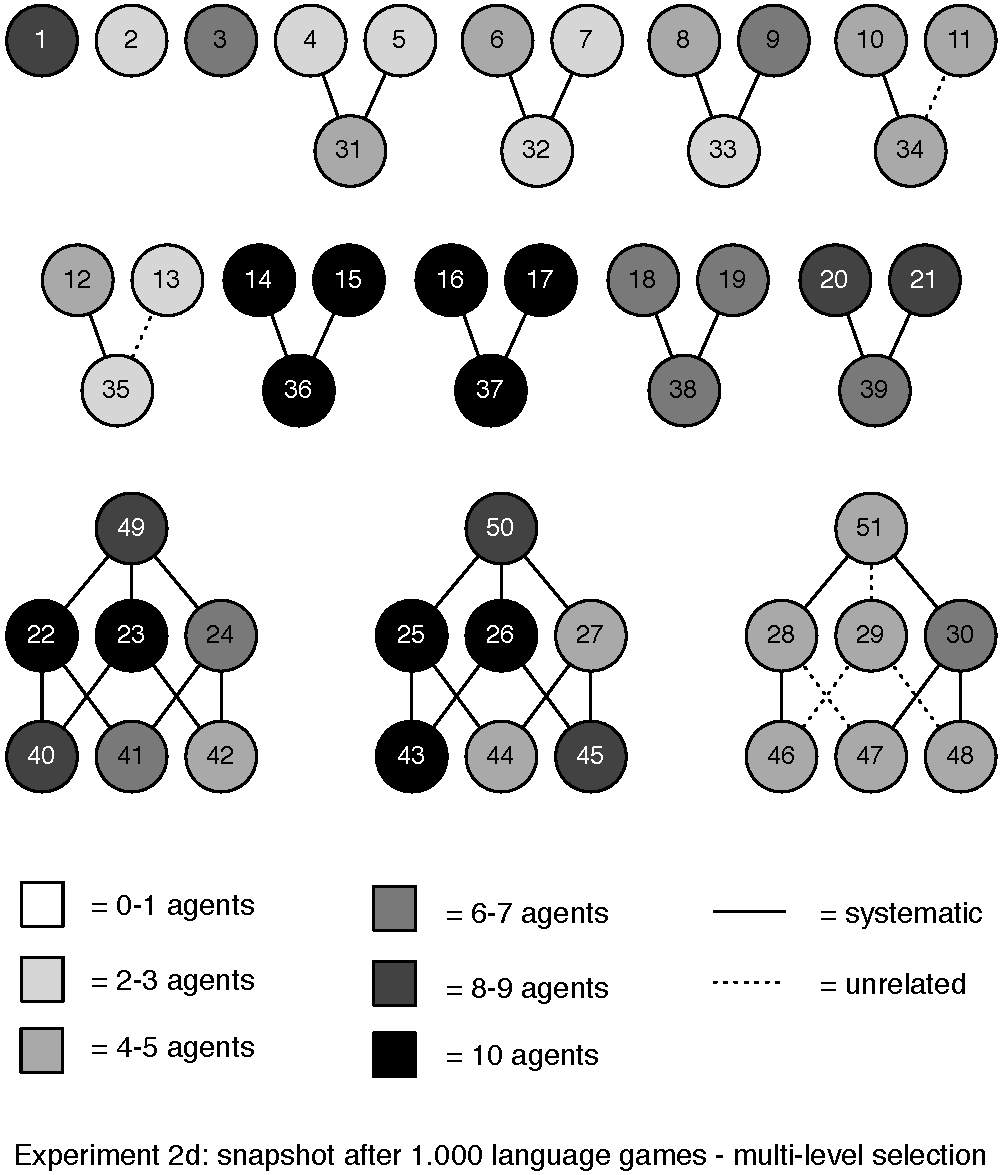
\includegraphics[width=0.7\textwidth]{Chapter4/figs/multilevel-coherence-no-analogy-1000}}
  \caption[Experiment 2: snapshot after 1.000 games (multi-level selection\is{multi-level selection})]{This diagram gives a snapshot of the average coherence in a population\is{speech population} of 10 agents after 1.000 language game\is{language game}s using the multi-level selection\is{multi-level selection} alignment strateg\is{alignment strategy}y. Compared to the simulations using direct selection, the agents seem to be converging more rapidly on meaning-form mappings and have already settled on 11 of them. Whereas there was no convergence at all yet for the more complex meanings 49--51 in the simulations using the direct selection alignment strateg\is{alignment strategy}y, here they are already shared by a majority of the population\is{speech population}. This suggests that multi-level selection\is{multi-level selection} speeds up the convergence dynamics significantly especially for related meanings. For the meanings in the bottom right, there is less systematicity\is{systematicity} and hence convergence takes longer time.}
   \label{f:2d-coherence-1000}
\end{figure}
\begin{figure}[p]
\centerline{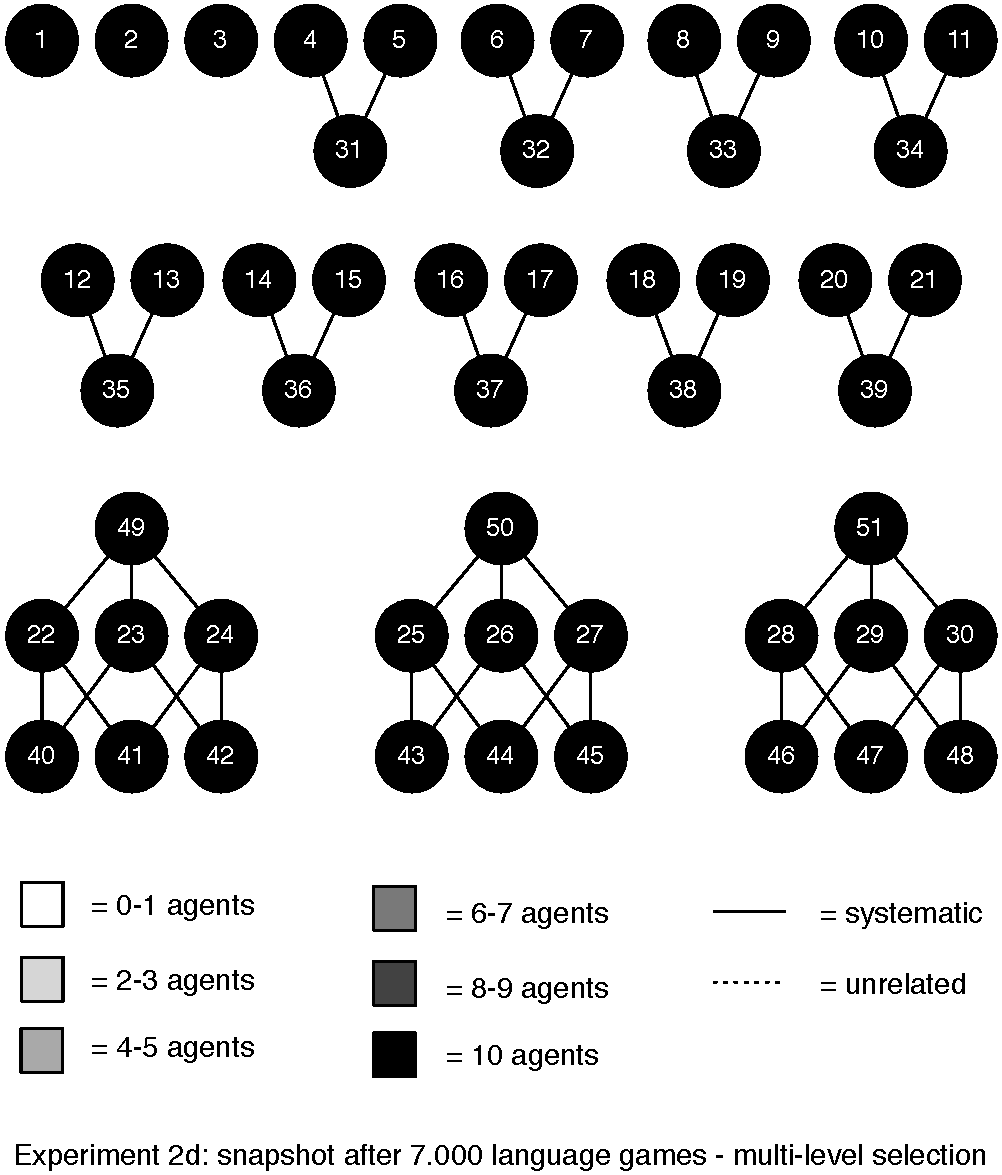
\includegraphics[width=0.7\textwidth]{Chapter4/figs/multilevel-coherence-no-analogy-7000}}
  \caption[Experiment 2: snapshot after 7.000 games (multi-level selection\is{multi-level selection})]{This diagram gives a snapshot of the average coherence in a population\is{speech population} of 10 agents after 7.000 language game\is{language game}s using the multi-level selection\is{multi-level selection} alignment strateg\is{alignment strategy}y. All the circles are black which means that the entire population\is{speech population} prefers the same meaning-form mappings. The language is also fully systematic so the agents have converged on 30 case marker\is{case!case marking}s which can be combined into 51 different constructions. The results indicate that even for instance-based\is{exemplar-based models} learners/innovat\is{innovation}ors systematicity\is{systematicity} can be reached by keeping a link between newly acquired constructions and the constructions that were used for learning or creating them.}
   \label{f:2d-coherence-7000}
\end{figure}


\subsubsection{Discussion}
 The results show that the agents reach full systematicity\is{systematicity} if each level in the linguistic inventor\is{linguistic inventory}y can have an influence on the competit\is{competition}ion in other levels. It is now important to understand why this is the case and why the other alignment strateg\is{alignment strategy}ies did not yield full systematicity\is{systematicity}.

First of all, bottom-up selection doesn't improve on the results of experiment 1 in terms of convergence speed and it doesn't lead to a systematic mapping of meaning to form across patterns. A closer examination of the the alignment strateg\is{alignment strategy}y reveals that the relatively high systematicity\is{systematicity} of 80\% is due to the higher frequency\is{frequency} of single-argument constructions. The frequent use of these constructions each time has repercussions for the competit\is{competition}ion between larger constructions whereas this is not the case in the other direction. If there would be more patterns than single-argument constructions, the improvement would therefore be less high. The patterns that resist the bottom-up selection can do so because the competit\is{competition}ion is not fully decided yet on a lower level (each time reinforc\is{reinforcement}ing competing patterns) and there is additional competit\is{competition}ion on the level of the patterns themselves which may have different winners than those on lower levels. In the end, though, the bottom-up strategy should lead to full systematicity\is{systematicity} but only very slowly and because the smaller constructions are more frequent.

The top-down strategy is affected by frequency\is{frequency} as well: competit\is{competition}ion between the larger constructions has significant impact on lower levels because it can increase the scores of up to six constructions while at the same time punishing all competit\is{competition}ors. However, since the smaller constructions are actually more frequent than the larger ones, some divergent competit\is{competition}ion pathways may resist this influence from the patterns and survive nevertheless. As the results indicate, this in fact happens in most of the simulations. Top-down selection thus improves systematicity\is{systematicity} significantly, but it is affected by the frequency\is{frequency} of the various levels of linguistic items and it is therefore no guarantee of full systematicity\is{systematicity}.

Finally, the agents can achieve full systematicity\is{systematicity} through multi-level selection\is{multi-level selection}. This strategy allows the competit\is{competition}ion of each level to influence the competit\is{competition}ion on others and given its n-directionality, it is not (or less) dependent on differences in frequency\is{frequency}. Moreover, the agents do not need to differentiate between a `higher' and a `lower' level but can treat all links between constructions on equal footing. The results of experiment 2 confirm earlier results on multi-level selection\is{multi-level selection} and systematicity\is{systematicity} reported by \citet{steels07multilevel}. In these experiments, which involved a scale-up in convergence space, multi-level selection\is{multi-level selection} outperforms the other strategies even more significantly.

\section{Experiment 3: multi-level selection\is{multi-level selection} with analog\is{analogy}y}
\label{s:pattern-exp-3}

Similarly to the previous experiments, experiment 3 investigates how baseline experiment 3 can be extended with a diagnostic\is{learning strategies!diagnostics} and repair\is{learning strategies!repair strategies} for pattern formation\is{formation}\is{pattern formation}. Since the previous experiments identified the problem of systematicity\is{systematicity}, experiment 3 first of all needs to verify whether the conclusions of the second experiment also hold for the new set-up in which the agents are capable of performing analog\is{analogy}ical reasoning over events. I will then report an experiment that adapts the algorithm for multi-level selection\is{multi-level selection} to the token-frequency\is{frequency} alignment strateg\is{alignment strategy}y of baseline experiment 3d (see section \ref{s:base3}).

\subsection{Experimental set-up}

Experiment 3 features the same experimental set-up as baseline experiment 3 with the addition of a diagnostic\is{learning strategies!diagnostics} and repair\is{learning strategies!repair strategies} strategy for pattern formation\is{formation}\is{pattern formation}. To summarize:

\begin{itemize}
\item The population\is{speech population} consists of 10 agents that engage in description game\is{language game!description game}s;
\item The meaning space is the same one as detailed in Table \ref{t:events} and all event type\is{event type}s occur with the same frequency\is{frequency};
\item The agents have two diagnostic\is{learning strategies!diagnostics}s: detecting unexpressed variable equal\is{variable equality}ities and the new diagnostic\is{learning strategies!diagnostics} detecting whether two constructions were applied during processing;
\item The agents have two repair\is{learning strategies!repair strategies} strategies: one for inventing and learning new verb\is{verb}-specific marker\is{case!case marking}\is{case!case marking}s and one for combining these marker\is{case!case marking}\is{case!case marking}s into a larger construction. The invention and learning strategy also includes the possibility of exten\is{extension}ding and reusing\is{reuse} existing marker\is{case!case marking}\is{case!case marking}s through analog\is{analogy}ical reasoning. The algorithm for analog\is{analogy}y is the same as in baseline experiment 3 and only looks at individual marker\is{case!case marking}\is{case!case marking}s.
\end{itemize}

The experiment has been tested using five different alignment strateg\is{alignment strategy}ies. The first four strategies are individual selection, top-down selection, bottom-up selection and multi-level selection\is{multi-level selection} using the same fine-grained lateral inhibition\is{lateral inhibition} mechanism as used in baseline experiment 3c. This means that competit\is{competition}ion is only held at the level of the co-occur\is{co-occurrence}rence links between a construction and a lexical entry rather than at the level of the constructions themselves. The algorithms can be summarized as follows:

\begin{itemize}
\item {\bfseries Individual selection:} This is the exact same set-up as baseline experiment 3c. If a game was successful, the hearer will increase the score of the co-occur\is{co-occurrence}rence link between the applied lexical entry and the applied construction(s) by 0.1. He will also decrease the scores of the competing links by 0.1. The score of a link is always between 0 (high uncertainty) and 1 (high confidence\is{confidence}).
\item {\bfseries Top-down selection:} In this strategy, the hearer will not only increase the score of the relevant co-occur\is{co-occurrence}rence link, but also the score of all the co-occur\is{co-occurrence}rence links that link the lexical entry to the smaller constructions which are related to the applied construction. The scores of the competit\is{competition}ors of these links are decreased.
\item {\bfseries Bottom-up selection:}  In this strategy, the hearer increases the score of the relevant link and of all the co-occur\is{co-occurrence}rence links that link the lexical entry to the larger constructions which are related to the applied constructions. All competit\is{competition}ors of these links are punished.
\item {\bfseries Multi-level selection\is{multi-level selection}:} In this strategy, the hearer increases the scores of the relevant co-occur\is{co-occurrence}rence links and of all the links which link the lexical entry to constructions that are related to the applied constructions.
\end{itemize}

The fifth experimental set-up does not involve lateral inhibition\is{lateral inhibition} but implements {\bfseries multi-level selection\is{multi-level selection} and memory decay\is{memory decay}}. In this set-up, the hearer will not only increase the frequency\is{frequency} score of the applied constructions, but also that of all the related constructions by 1. The frequency\is{frequency} scores have no upper limit, so the higher the score, the more entrench\is{entrenchment}ed the construction is. After an agent has individually engaged in 200 language game\is{language game}s, the frequency\is{frequency} scores of all the items in the inventory are decreased.

In all five set-ups, the speaker will use the co-occur\is{co-occurrence}rence links to speed up processing. This means that not the entire inventory of constructions is considered, but only those constructions which are linked to the lexical entry. Links can be added through co-occur\is{co-occurrence}rence. When the speaker is faced with multiple hypotheses, he will choose the construction which either has the strongest co-occur\is{co-occurrence}rence link with the lexical entry (in the first four set-ups) or the one with the highest token frequency\is{token frequency}\is{frequency} (in the fifth set-up). During processing, only the scores of individual competit\is{competition}ors are taken into account. All simulations have been run in 10 series of 12.000 language game\is{language game}s.

\subsection{Results and discussion}

In this section, the first four set-ups are again compared to each other to demonstrate the reoccurrence of the problem of systematicity\is{systematicity}. The fourth set-up (multi-level selection\is{multi-level selection} with lateral inhibition\is{lateral inhibition}) is then compared more thoroughly to the fifth set-up using multi-level selection\is{multi-level selection} and memory decay\is{memory decay}. Finally, this section offers a closer look at one language evolved using the fifth set-up.

\begin{figure}[p]
\centerline{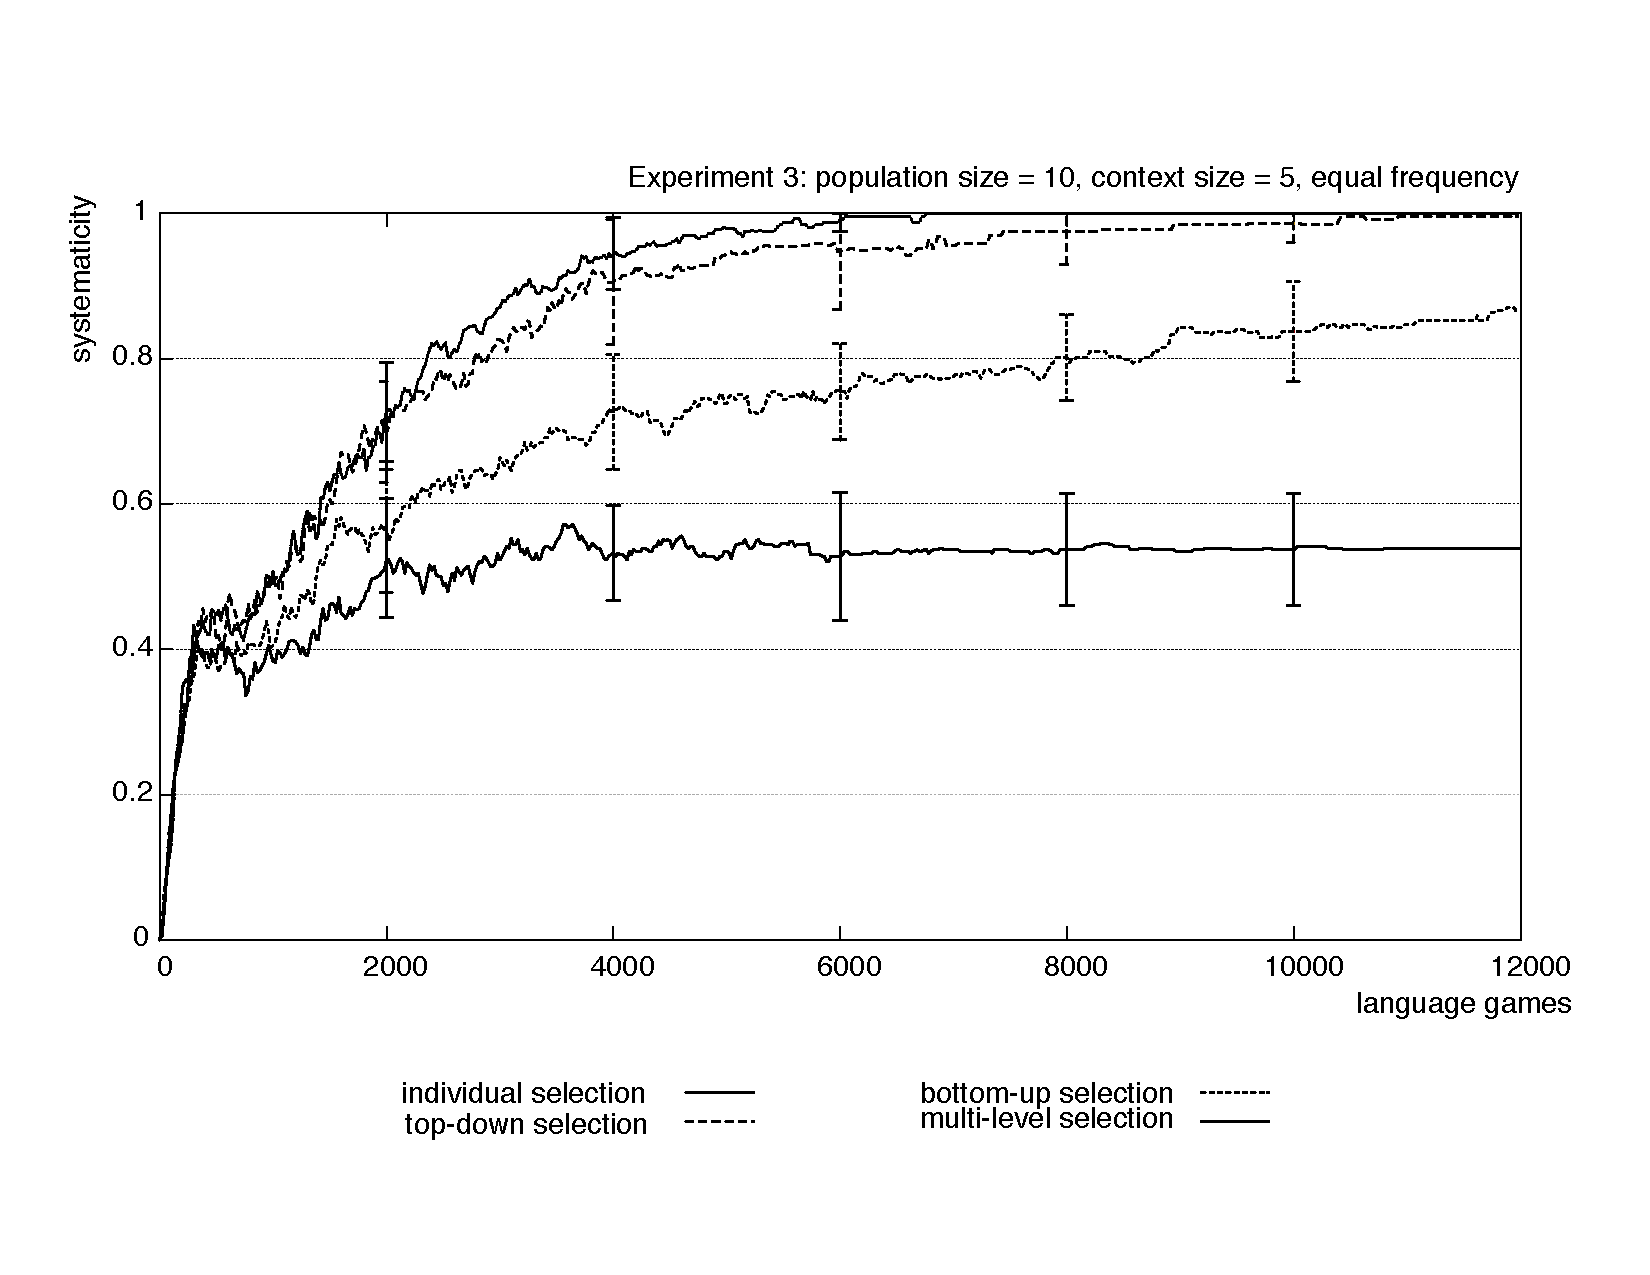
\includegraphics[width=\textwidth]{Chapter4/figs/systematicity3}}
  \caption[Experiment 3: systematicity]{This graph compares systematicity\is{systematicity} in the first four experimental set-ups of experiment 3. The results confirm those of experiment 2. Even though there is potentially less variation\is{variation} because of the reuse\is{reuse} of existing marker\is{case!case marking}s, individual selection stagnates at 50\% systematicity\is{systematicity}. Bottom-up selection increases systematicity\is{systematicity} beyond 80\% but also gets stuck. Top-down selection manages to reach full systematicity\is{systematicity} in more simulations than in experiment 2 because of the smaller variation\is{variation} space, but does not guarantee full systematicity\is{systematicity}. Only multi-level selection\is{multi-level selection} reaches systematicity\is{systematicity} in all the simulations and does so significantly faster than the other alignment strateg\is{alignment strategy}ies.}
   \label{f:systematicity3}
\end{figure}


\subsubsection{Results}
 Figure \ref{f:systematicity3} compares the first four experimental set-ups to each other in terms of systematicity\is{systematicity}. The lines indicating systematicity\is{systematicity} for each set-up show the same behaviour as those in experiment 2 (Figure \ref{f:systematicity2}). The first set-up using the alignment strateg\is{alignment strategy}y of individual selection fluctuates between 45 and 60\% systematicity\is{systematicity} and stops evolving after 6.000 language game\is{language game}s. The bottom-up strategy reaches more than 80\% systematicity\is{systematicity} after 8.000 language game\is{language game}s. In some simulations, this strategy leads up to 90\% but never to maximum systematicity\is{systematicity}. Top-down selection performs a bit better than in experiment 2 due to the fact that the agent's capacity of reusing\is{reuse} existing marker\is{case!case marking}s leads to a smaller variation\is{variation} space so `frozen accidents' are less likely. Yet, as the results show, some simulations still involve an unsystematic convention\is{convention} and reaching systematicity\is{systematicity} takes a longer time than the multi-level selection\is{multi-level selection} strategy. The latter strategy is again the only one which leads to full systematicity\is{systematicity} in all the simulations.

\begin{figure}[p]
\centerline{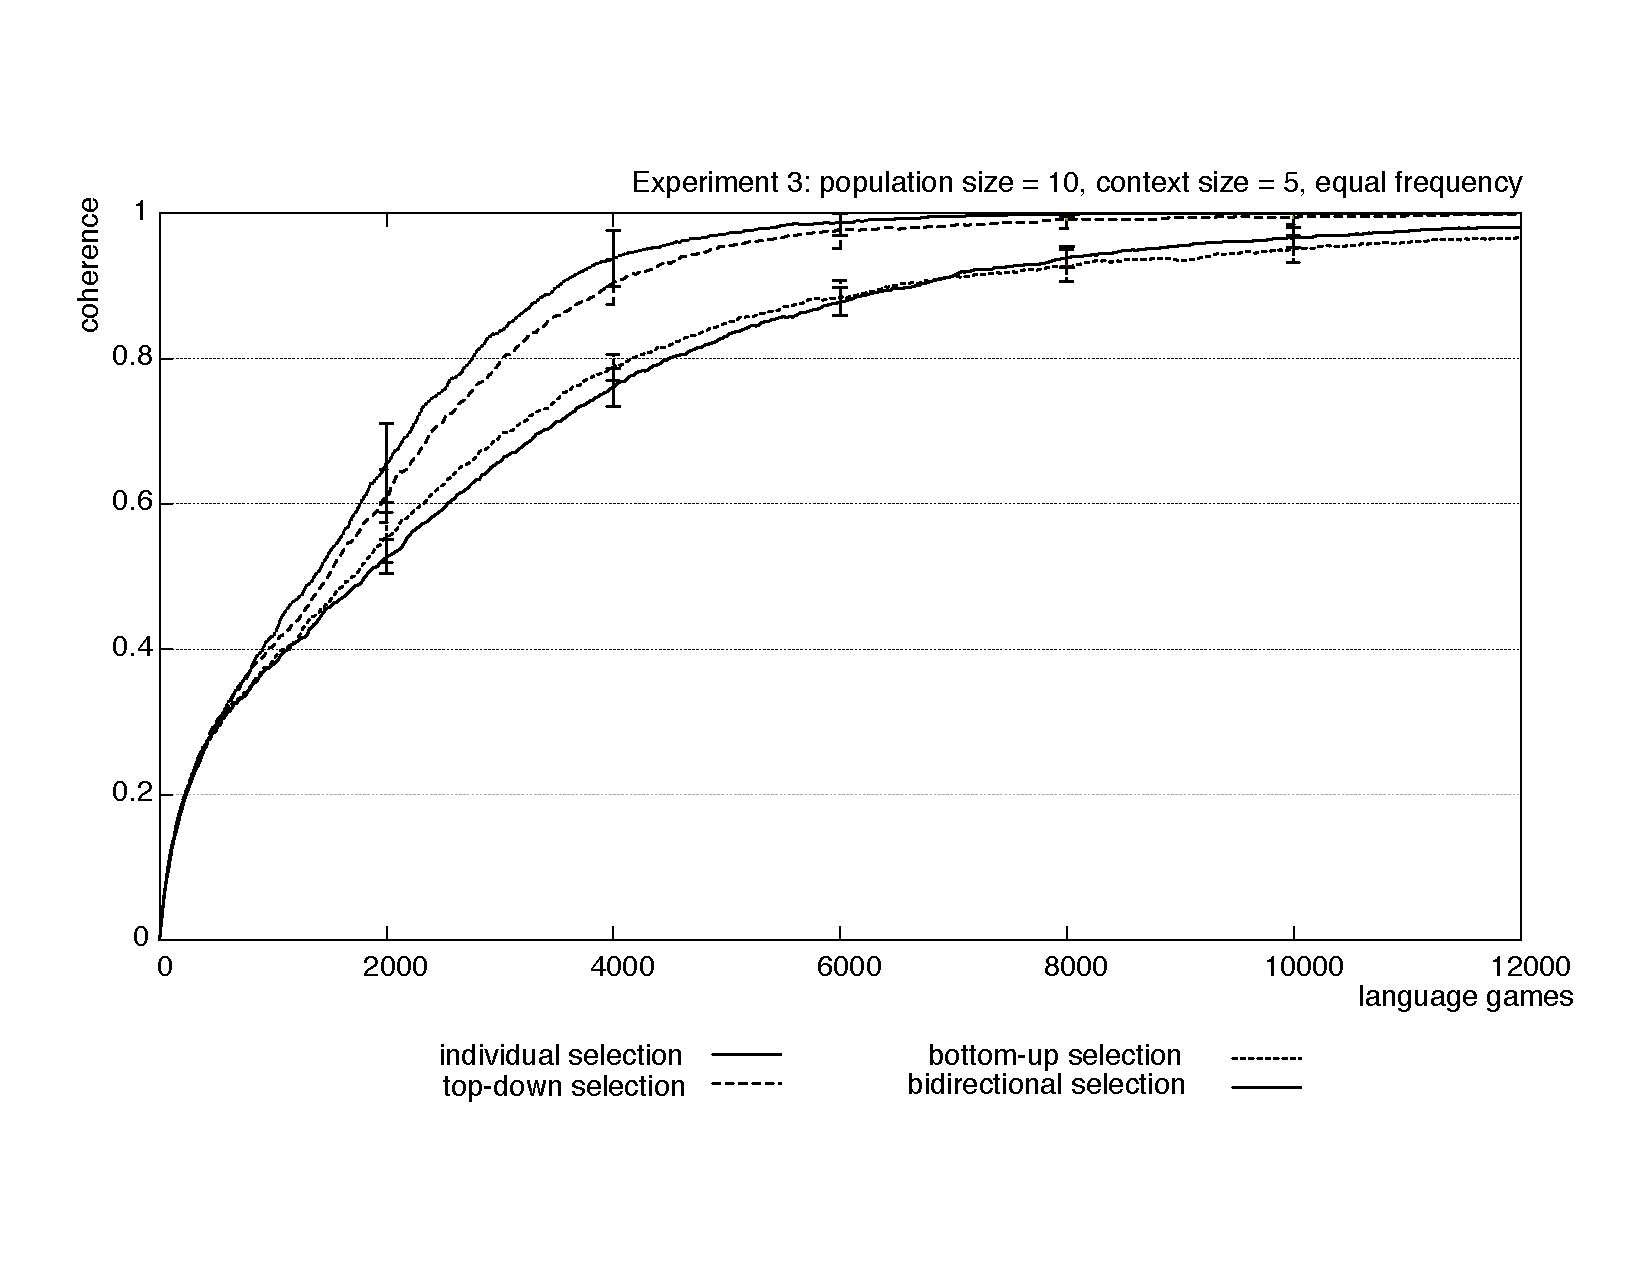
\includegraphics[width=\textwidth]{Chapter4/figs/coherence3}}
  \caption[Experiment 3: coherence]{This graph compares the first four set-ups of experiment 3 in terms of meaning-form coherence. The graph shows that multi-level and top-down selection perform equally well and reach 100\% between 6.000 and 8.000 language game\is{language game}s. Bottom-up and individual selection again run almost parallel and reach coherence faster than in experiment 2 because of the smaller variation\is{variation} space.}
   \label{f:coherence3}
\end{figure}

The four set-ups also confirm the results of experiment 2 in terms of coherence. Figure \ref{f:coherence3} shows that bottom-up selection and individual selection again run almost parallel in terms of convergence. This time the agents reach coherence faster because of the smaller variation\is{variation} space. Multi-level and top-down selection also perform equally well and reach coherence between 6.000 and 8.000 language game\is{language game}s.

\begin{figure}[t]
\centerline{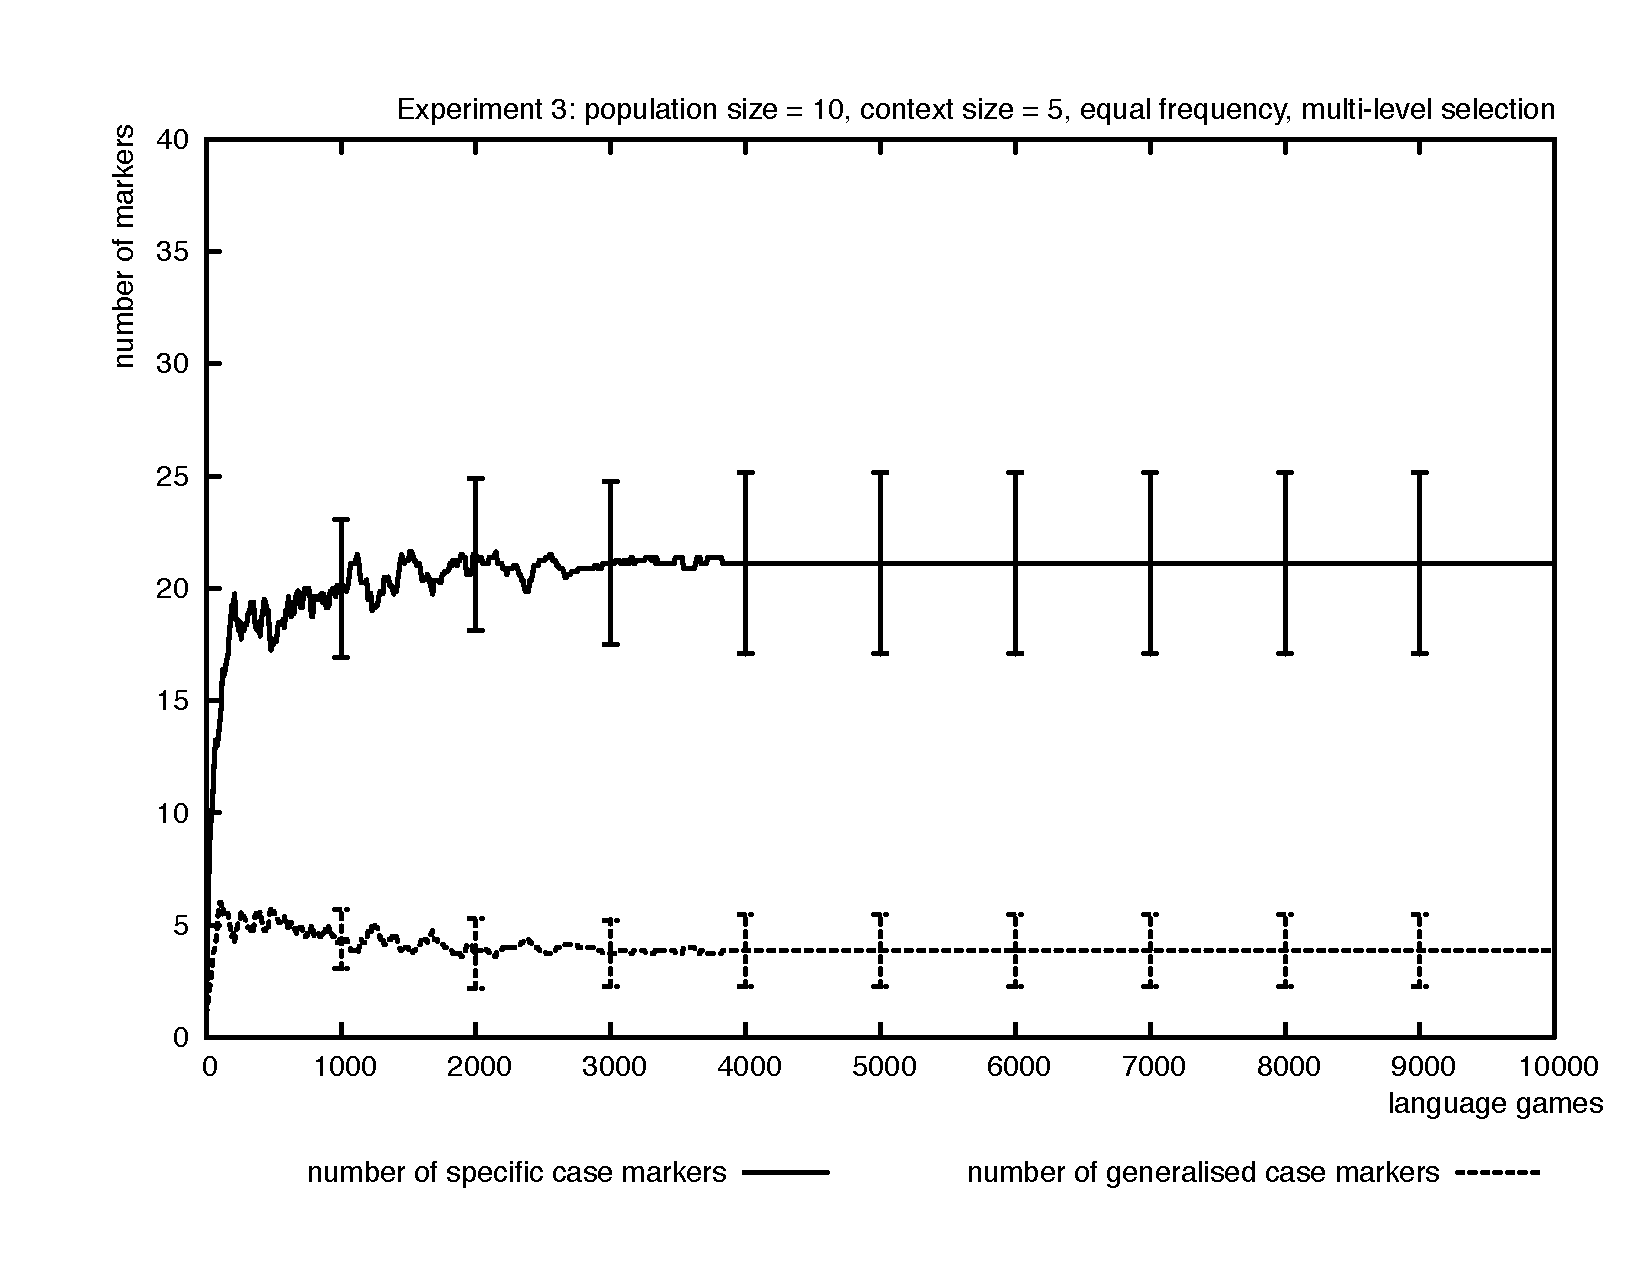
\includegraphics[width=\textwidth]{Chapter4/figs/markers3}}
  \caption[Experiment 3: number of markers]{This graph shows the average number of marker\is{case!case marking}s known by each agent using the strategy of multi-level selection\is{multi-level selection} with lateral inhibition\is{lateral inhibition} (the fourth set-up of experiment 3). The results show that the generalization rate of the agents is not impressive: only 3-5 semantic roles survive the competit\is{competition}ion as opposed to 18-25 specific marker\is{case!case marking}s.}
   \label{f:markers3}
\end{figure}

Figure \ref{f:markers3} gives an indication of the kinds of languages that are formed in the population\is{speech population} if the agents use the fourth set-up (multi-level selection\is{multi-level selection} with lateral inhibition\is{lateral inhibition}). The graph shows that the generalization rate of the agents is not really impressive: only three to five generaliz\is{generalization}ed roles survive the competit\is{competition}ion. Moreover, these roles only cover two or maximally three participant roles. This is clear from the fact that there are still 18 to 25 specific marker\is{case!case marking}s floating around in the population\is{speech population}.

\begin{figure}[p]
\centering
\begin{tabular}{c}
{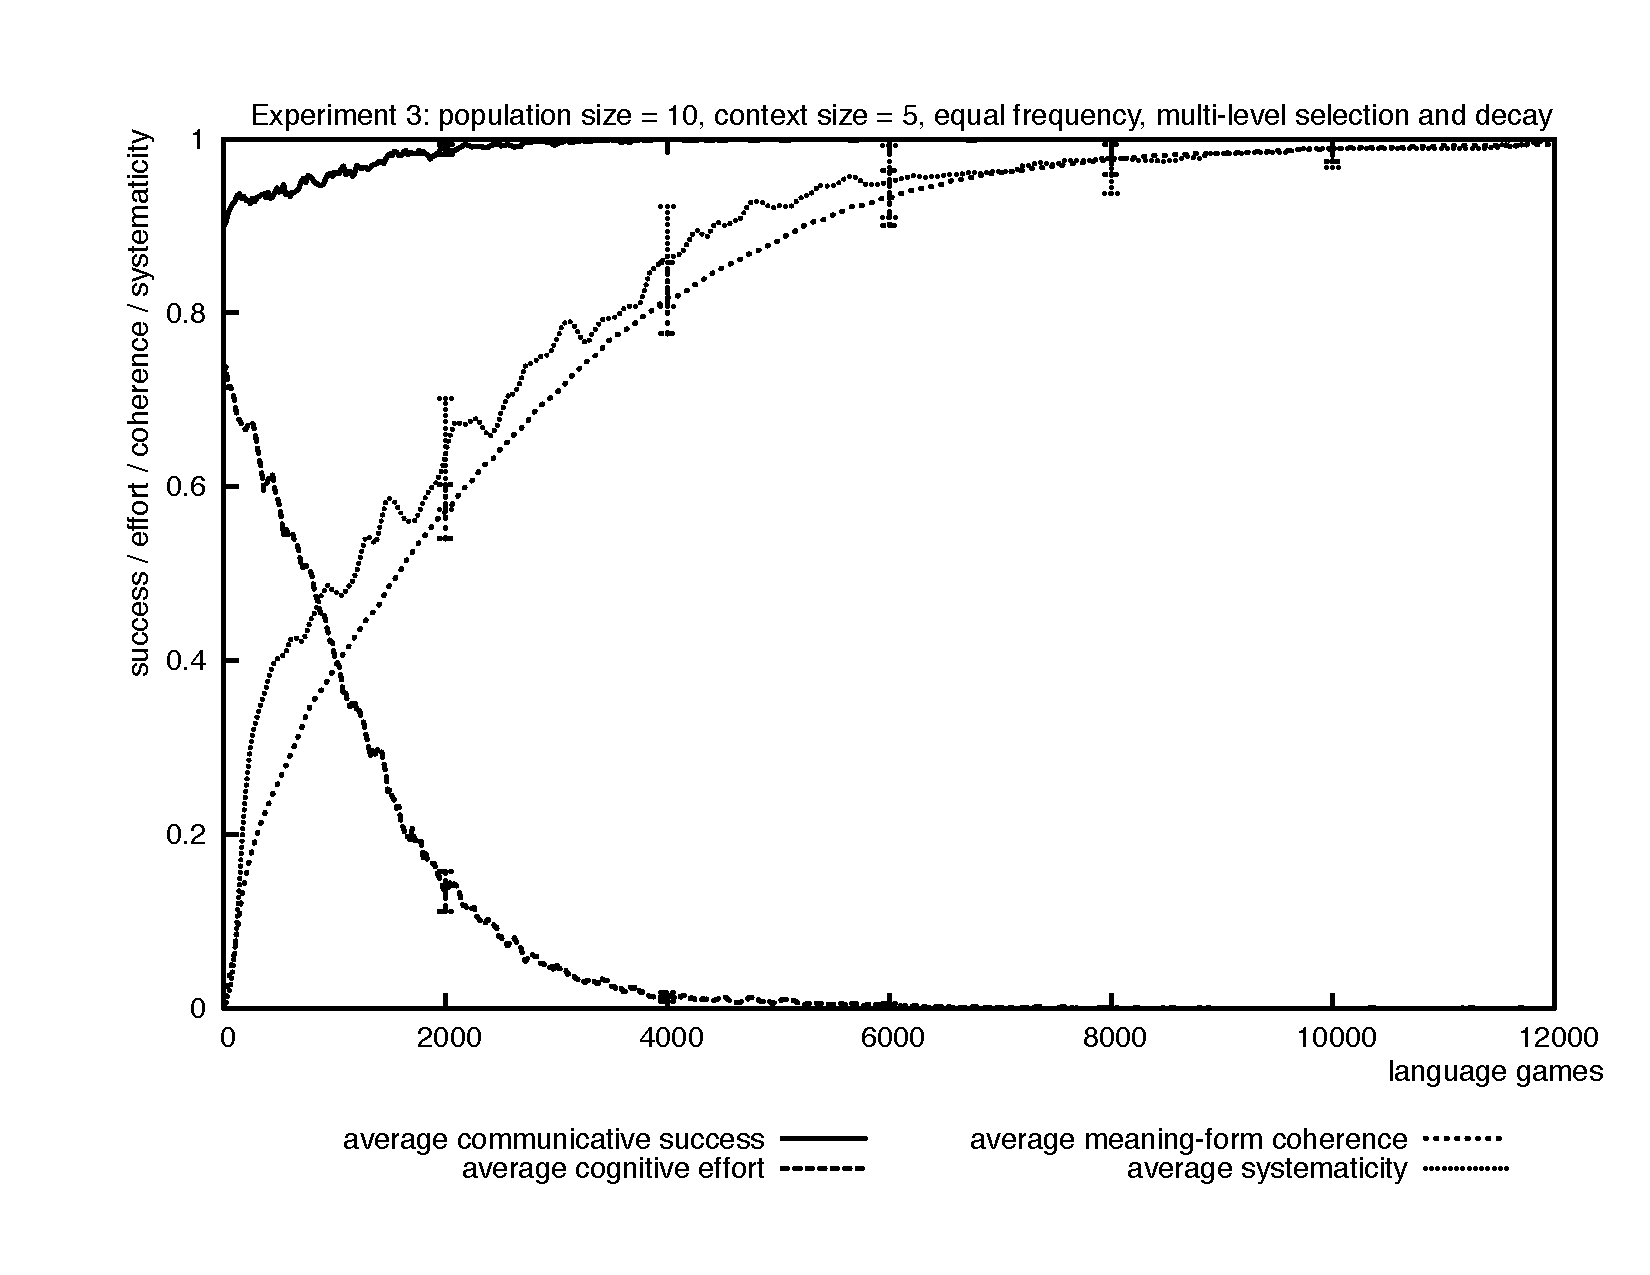
\includegraphics[width=0.8\textwidth]{Chapter4/figs/systematicity3b}}
\\
{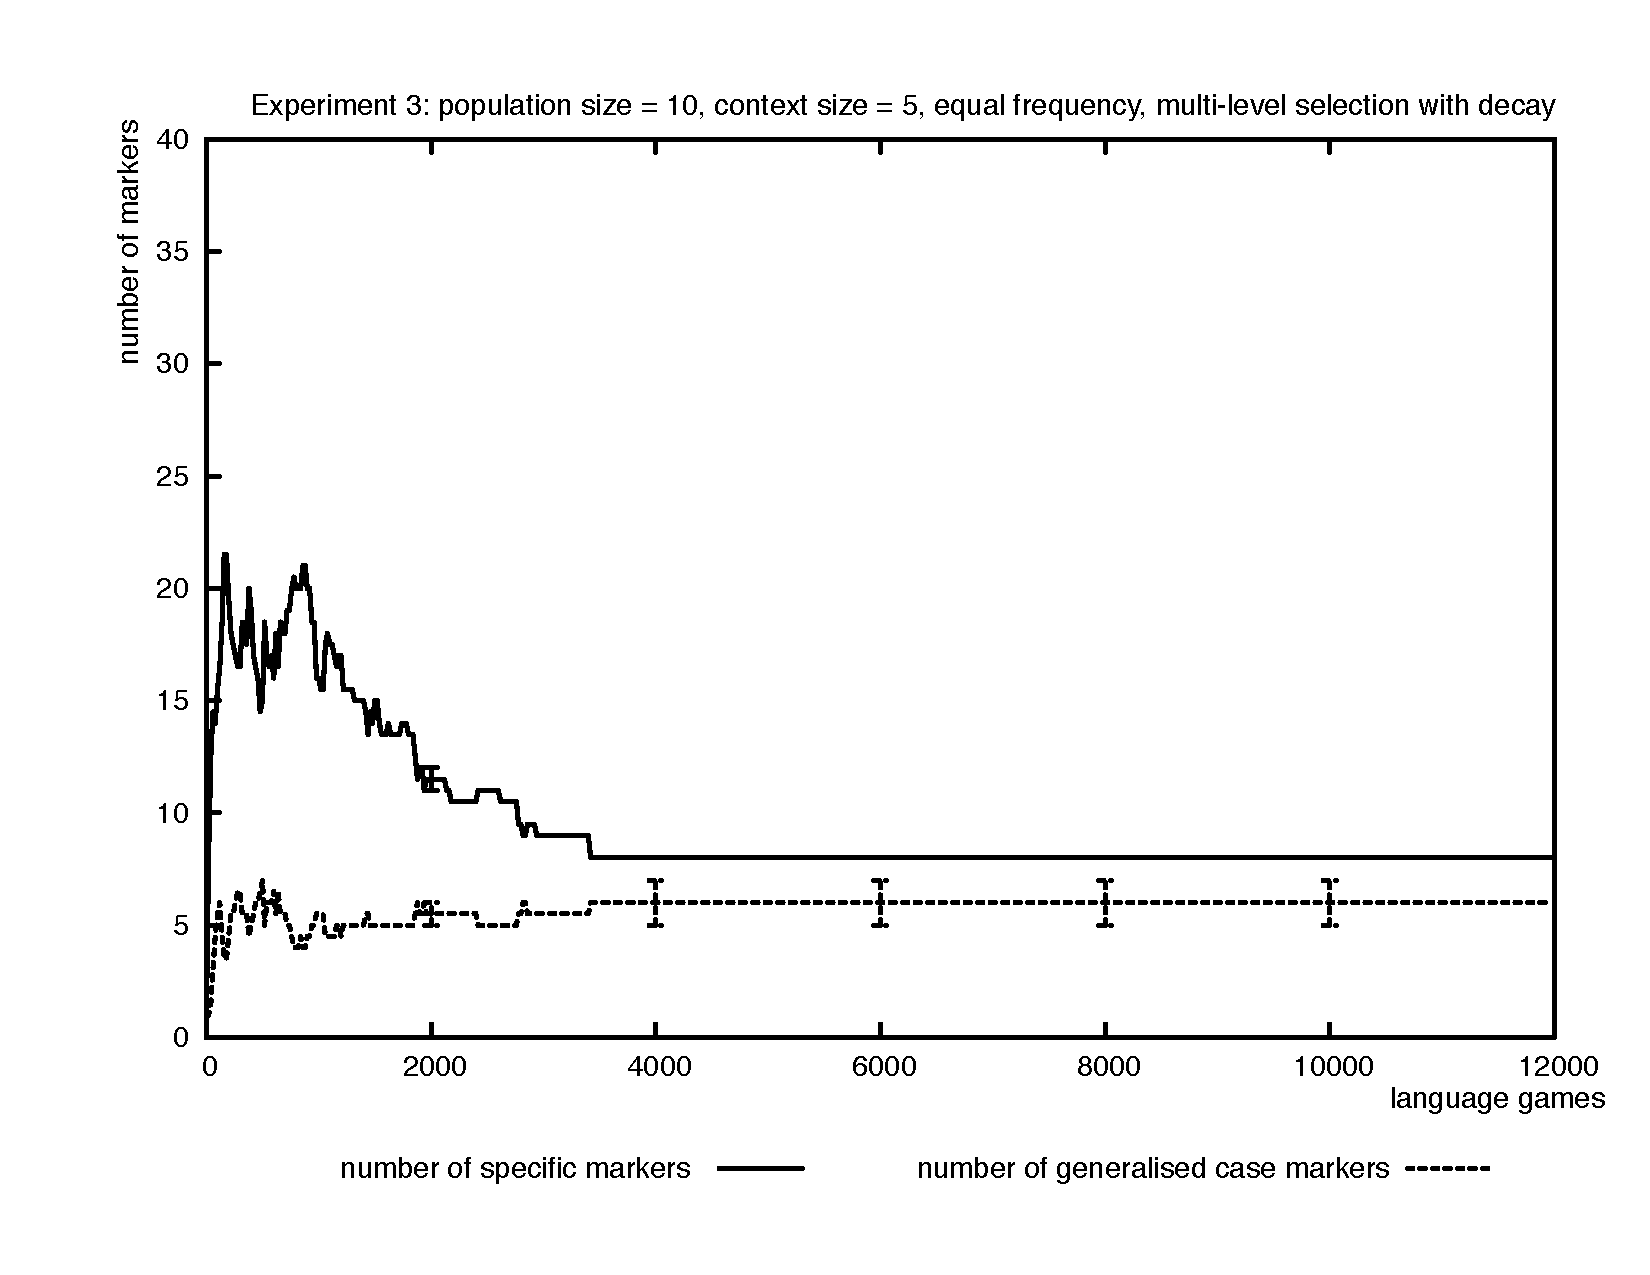
\includegraphics[width=0.8\textwidth]{Chapter4/figs/markers3-decay}}
\end{tabular}
\caption[Experiment 3: results for set-up 4]{The top graph shows communicative success\is{communicative success}, cognitive effort\is{cognitive effort}, systematicity\is{systematicity} and meaning-form coherence in the set-up using multi-level selection\is{multi-level selection} and decay. The bottom graph shows the average number of marker\is{case!case marking}s in the same set-up.}
\label{f:multi-level-decay}
\end{figure}

These results can be compared to the performance\is{performance} of the fifth set-up (multi-level selection\is{multi-level selection} with decay) which is illustrated in Figure \ref{f:multi-level-decay}. The top graph shows the results for communicative success\is{communicative success}, cognitive effort\is{cognitive effort}, meaning-form coherence and systematicity\is{systematicity}. As the graph indicates, the agents succeed in reaching full systematicity\is{systematicity} somewhere between 8.000 and 12.000 language game\is{language game}s, which is a bit slower than the alignment strateg\is{alignment strategy}y using lateral inhibition\is{lateral inhibition}. The bottom graph shows the average number of marker\is{case!case marking}s floating around in the population\is{speech population}. Here, we see that the average number of specific marker\is{case!case marking}s has made a significant drop from 18-25 marker\is{case!case marking}s to only 9. The number of semantic roles shifts from simulation to simulation between 4 and 6. The semantic roles also tend to be more general categories than in the simulations using lateral inhibition\is{lateral inhibition}.


Here is a list of marker\is{case!case marking}s and the participant roles they cover in one of the simulations (from more general to more specific):

\begin{itemize}
\item {\em -kad:} object-1, approach-1, fall-1, touch-1, move-outside-1
\item {\em -fuir:}  grasp-2, hide-2, move-inside-2, touch-2, walk-to-1
\item {\em -kazo:} approach-2, fall-2, grasp-1, hide-1, walk-to-2
\item {\em -hesa:} move-1, take-3
\item {\em -ti:} visible-1, take-1
\item {\em -qiwo:} move-inside-1, give-3
\item {\em -fen:} distance-decreasing-1
\item {\em -rem:} distance-decreasing-2
\item {\em -gaeh:} move-outside-2
\item {\em -wupu:} cause-move-on-1
\item {\em -chuiw:} cause-move-on-2
\item {\em -nuip:} cause-move-on-3
\item {\em -tu:} give-1
\item {\em -hozae:} give-2
\item {\em -fut:} take-2
\end{itemize}

The above marker\is{case!case marking}s occur systematically across patterns for marking the same parti\-ci\-pant roles. In this specific example, the agents succeeded in reaching coherence and systematicity\is{systematicity} after only 8.000 language game\is{language game}s. When we compare the results to those of baseline experiment 3d, roughly the same level of generalization is reached.

\begin{figure}[p]
\centerline{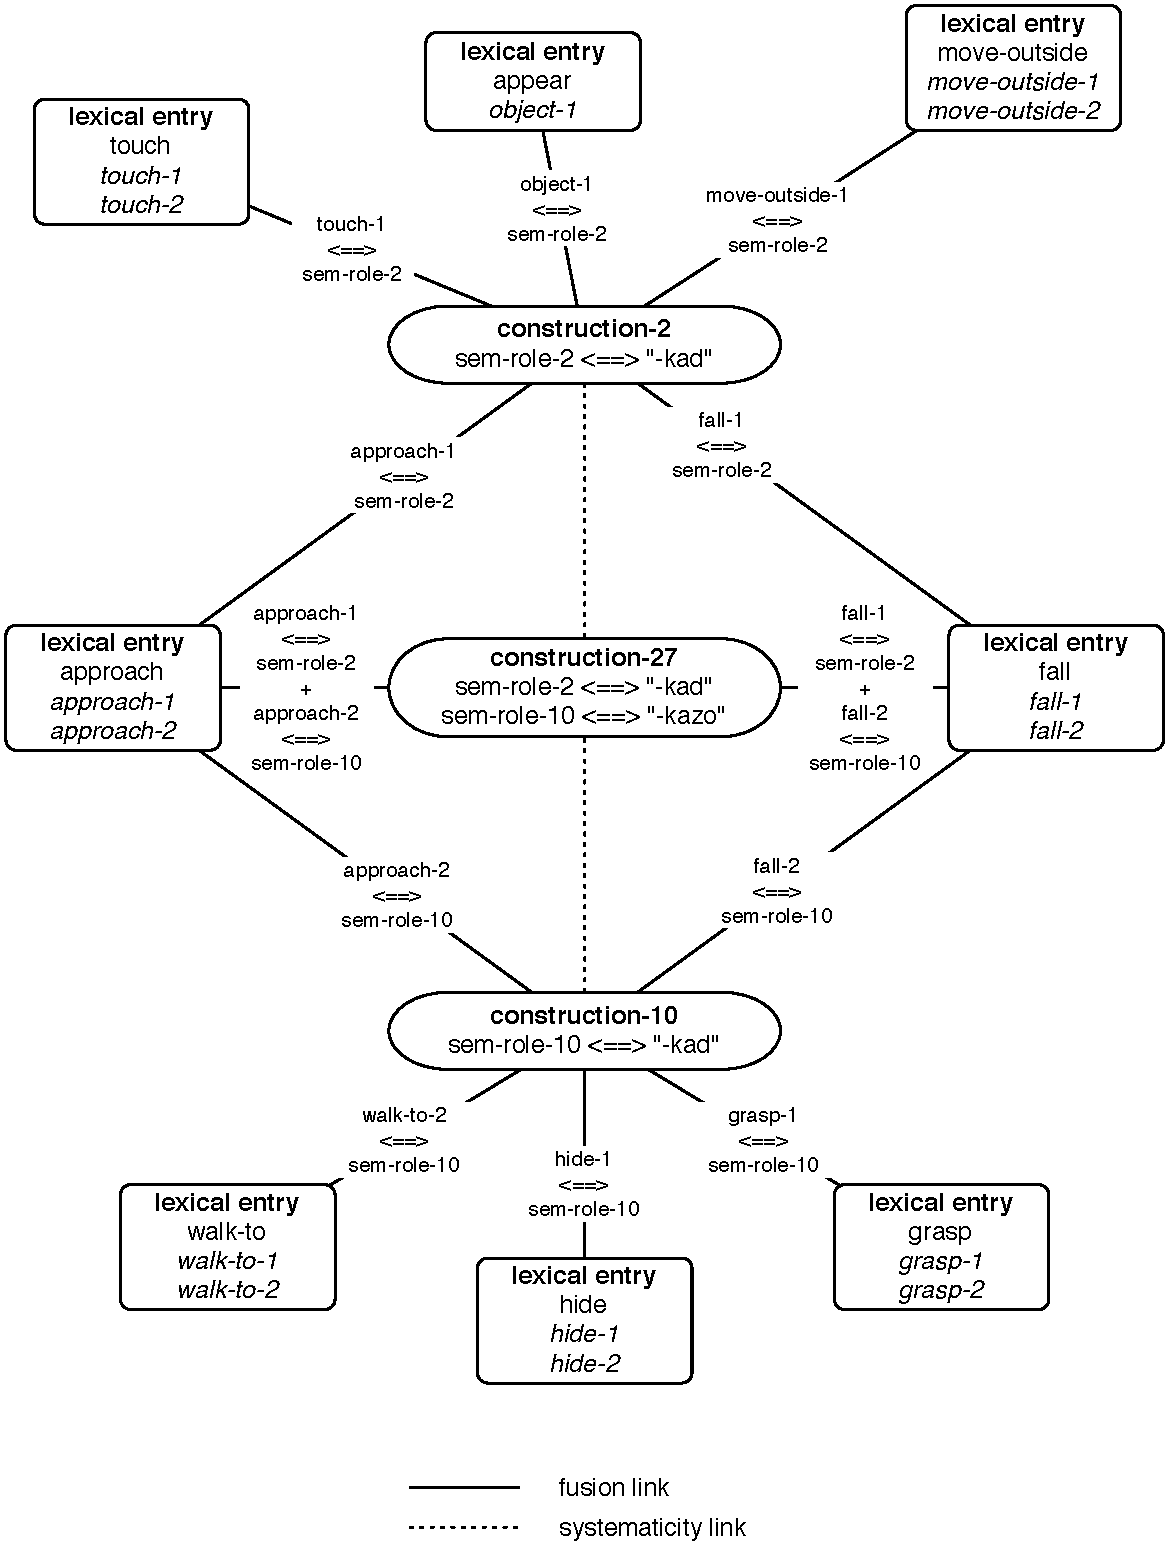
\includegraphics[width=0.75\textwidth]{Chapter4/figs/network}}
  \caption[Experiment 3: a partial network of set-up 5]{This figure gives a partial network for one agent in one of the simulations using multi-level selection\is{multi-level selection} with decay. In the middle there are three constructions which are systematically related to each other. The constructions are also linked with lexical entries. The links act both as co-occur\is{co-occurrence}rence links for optimizing processing and as fusion\is{fusion} links for integrating the participant roles of the lexical entries with the semantic roles of the constructions. The networks are constructed in a stepwise fashion as a response to communicative needs.}
   \label{f:network}
\end{figure}

Finally, Figure \ref{f:network} looks inside the linguistic inventor\is{linguistic inventory}y of a single agent and offers a partial network of the agent's knowledge of its language. The figure concentrates on three constructions (in the middle) which are related to each other (indicated by the dotted line). The relation between the constructions indicate that construction-27 was created as a pattern of construction-2 and construction-10. The figure also shows all the lexical entries that are convention\is{convention}ally associated with these constructions. The links between the lexical entries and the constructions are used for optimizing processing: instead of trying out all the constructions in memory, only the linked constructions are considered. Links can be added as part of a problem-solving\is{problem-solving} process during communication or pruned if the co-occur\is{co-occurrence}rence is not a successful one. Some redundant co-occur\is{co-occurrence}rence links may survive in the inventory. The links can also be seen as fusion\is{fusion} links: they are annotated with information on how the participant roles can be fused with the semantic roles of the construction. This annotation is however not used by the agents themselves but for the clarity of interpretation for the experimenter. The actual fusion\is{fusion} is taken care of by the unification\is{unification} of the potential valents of the lexical entry with the actual valency of the construction.


\subsubsection{Discussion}
 The results of experiment 3 confirm the problem of systematicity\is{systematicity} that was uncovered in the other experiments. Here too, the strategy using multi-level selection\is{multi-level selection} was the only one to yield fully systematic languages. The systematicity\is{systematicity} rate was in each of the first four set-ups comparable to the rates in experiment 2. This may come as a surprise since the variation\is{variation} space is potentially smaller because the agents can exten\is{extension}d the use of existing marker\is{case!case marking}s rather than inventing new ones all the time.

A closer look at the number of marker\is{case!case marking}s in the fourth set-up (multi-level selection\is{multi-level selection} with lateral inhibition\is{lateral inhibition}), however, pointed to the reason for the small differences in systematicity\is{systematicity} rates: only a very small number of semantic roles survived the competit\is{competition}ion compared to a large number of specific marker\is{case!case marking}s. This means that the generalization rate is not really impressive so the number of variation\is{variation}s is not much smaller in these simulations than was the case in experiment 2. The resulting number of specific mar\-kers versus semantic roles corresponds to the results obtained in baseline experiment 3c and also the reason for the result is the same: since the competit\is{competition}ion is held at the level of co-occur\is{co-occurrence}rence links and not at the level of constructions, the type frequency\is{type frequency}\is{frequency} of a marker\is{case!case marking} does not translate into a larger category gravity\is{category gravity}. Competition is held only in a local context so specific mar\-kers have an equally high chance of winning as more generaliz\is{generalization}ed semantic roles.

The results of the fifth set-up (multi-level selection\is{multi-level selection} with memory decay\is{memory decay}) also confirm the results of the baseline experiments and improve significantly in terms of generalization over the simulations using the fine-grained lateral inhibition\is{lateral inhibition} dynamics. The number of specific categories has dropped by half and larger, more general semantic roles have a selectionist advantage because they occur more often. The generalization rate roughly matches the performance\is{performance} of baseline experiment 3d.

The consistency in number of generaliz\is{generalization}ed semantic roles and specific marker\is{case!case marking}s across the baseline experiments and the pattern experiments indicate that this is the maximum generalization rate that the agents can reach. Possible improvements would have to come from two sources:

\begin{enumerate}
\item The structure of the world: The capacity of analog\is{analogy}ical reasoning is heavily dependent on the structure of the world environment in which communication takes place. If the agents have to communicate about lots of events which show recurrent patterns in terms of visual primitives, they will be able to detect more analog\is{analogy}ies. If, however, the world is totally unstructured, the agents will come up with more specific marker\is{case!case marking}s than general semantic roles.
\item The capacity of analog\is{analogy}ical reasoning can be made more flexible. At the moment, the agents make a sharp distinction between what is analog\is{analogy}ous and what is not. A possible relaxation could be to only care about whether the mapping between a source\is{semantic role!source} role and a target role is discriminating enough for identifying the target role as well. Another possibility would be to use a similarity or a distance metric instead of the more rigid structural mapping that the agents currently use.
\end{enumerate}

Experiment 3 also shows the potential power of the combination of analog\is{analogy}ical reasoning, pattern formation\is{pattern formation} and multi-level selection\is{multi-level selection} respectively. First of all, analog\is{analogy}ical reasoning over the linguistic inventor\is{linguistic inventory}y can lead to an increasing generalization rate in the population\is{speech population}, as is also shown in several instance-based\is{exemplar-based models} approaches to language \citep{daelemans05memory, skousen89analogical}. These models also argue that a language can look rule-based from outside whereas in fact the generalization is distributed over the linguistic items in the inventory. This experiment shows that this observation also holds true for the case of the emergence\is{emergence} of grammar if multi-level selection\is{multi-level selection} is applied. Finally, the formation\is{formation} of patterns to improve processing can have dramatic effects on the grammar: the patterns increase the survival chances of its related items; and they may potentially exten\is{extension}d their use as well in later interactions. 

So far, I did not spend much attention to the efficiency of the formalization of argument realization proposed in Chapter \ref{c:ar}. In all the experiments presented in this Chapter and the previous one, the representation has proven to be flexible enough to deal with the enormous amount of {\bfseries uncertainty} that is inherent to the emergence\is{emergence} of new grammar convention\is{convention}s. In this case, the agents needed a flexible way of integrating lexical entries with constructions of various degrees of entrench\is{entrenchment}ment. Instead of copying all the possible case frames into a new entry, the formalization allowed the agents to constantly `mould' their lexical entries until a stable set of convention\is{convention}s had been negotiat\is{negotiation}ed. In this way, the competit\is{competition}ion of case marker\is{case!case marking}s could be held exclusively at the level of constructions instead of creating an additional competit\is{competition}ion on the lexical level for how these lexical entries should be integrated with the constructions. The lexical entries also integrated as easily with verb\is{verb}-specific construction\is{construction!verb-specific construction}s as with verb\is{verb}-class specific constructions.

The formalization was also flexible enough to deal with {\bfseries multiple argument realization}: the agents were capable of integrating a single lexical entry into multiple patterns or constructions without the need for deriv\is{derivation}ational rules or additional copies in the lexicon\is{lexicon}. Moreover, the lexical entries do not need to `profile' their participant roles: the actual valency of a verb\is{verb} is determined by the construction it integrates with. Preferences for certain patterns of argument realization could be captured in this formalization by assigning a frequency\is{frequency} score to the co-occur\is{co-occurrence}rence links of the lexical entries and the constructions that they are convention\is{convention}ally associated with.

One aspect that is still absent in the experiment is how the functions of the case marker\is{case!case marking}s start to influence each other once they start combining into patterns. At this moment, the meanings of the marker\is{case!case marking}s stay the same and patterning only influences their survival chances. Future work would thus have to include a way for the patterns themselves to evolve, which would also require the analog\is{analogy}y to use the patterns as the source domain for innovat\is{innovation}ion rather than focusing exclusively on single marker\is{case!case marking}s.

Including the patterns into the search domain could however lead to a huge hypo\-the\-sis space and a complexity measure is needed to verify whether the algorithm for analog\is{analogy}y can scale up to larger worlds while maintaining a reasonable processing time. If not, a possible alternative could be a nearest-neighbour\is{nearest-neighbour} algorithm which has already been successfully applied to various tasks in natural language processing\is{natural language processing}. In a comparison between Royal Skou\-sen's {\em Analogical Modeling\is{Analogical Modeling}} \citep{skousen89analogical} and {\em Memory-Based Language Processing\is{Memory-Based Language Processing}} \citep{daelemans05memory}, \citet{daelemans02comparing} shows that a relatively simple and efficient nearest-neighbour\is{nearest-neighbour} learner yields comparable and sometimes even better results than the costly algorithm  of Analogical Modeling\is{Analogical Modeling}. This observation seriously challenges the more traditional approach to analog\is{analogy}y and is highly relevant for the discussion of this work as well.

\section{Towards syntactic cases}
\label{s:pattern-exp-4}

The experiments so far have dealt with stages 1 to 3 in the development of case marker\is{case!case marking}s (see Chapter 1). The next step is the introduction of syntactic roles that group together two or more semantic roles. In this section, I will introduce a first experiment that investigates how the transition to stage 4 can be achieved and what can be learned from the results. I will then use the grammatical square\is{grammatical square} as a roadmap for future experiments.

\subsection{A first experiment}

As I argued in sections \ref{s:stage3} and \ref{s:stage4}, syntactic roles impose even more abstraction\is{abstraction} on the conceptualization\is{conceptualization} of specific events than semantic roles do. In natural languages, syntactic roles typically emerge when a category gradually starts exten\is{extension}ding its use until two cases merge into one class. In this first tentative experiment, I will scaffold\is{scaffold} the merger of cases and assume that a case marker\is{case!case marking} can exten\is{extension}d its use by subcategorization rather than by merging two roles. I will make this assumption\is{assumption} more clear in the following paragraphs.


\subsubsection{Experimental set-up}
 The experiment features the exact same set-up as the fourth set-up in experiment 3: the agents are capable of reusing\is{reuse} a marker\is{case!case marking} through analog\is{analogy}y and combining the marker\is{case!case marking}s into larger patterns. They employ the alignment strateg\is{alignment strategy}y of multi-level selection\is{multi-level selection} using lateral inhibition\is{lateral inhibition}. The main question of the experiment is whether the agents are capable of aligning their grammars, which form an abstract intermediary layer of semantic and syntactic roles which are not directly observable by the other agents.

The novelty of this particular set-up involves the idea of `reusing\is{reuse} as much as possible'. Roughly speaking, a speaker will reuse\is{reuse} an existing marker\is{case!case marking} even if it is not analog\is{analogy}ous to the target role, on the condition that the marker\is{case!case marking} does not cover a conflicting participant role yet. The algorithm is operationalized as follows:

\begin{enumerate}
\item If the speaker diagnosed a problem of unexpressed variable equal\is{variable equality}ities, he tries to repair\is{learning strategies!repair strategies} the problem.
\item The speaker checks whether he already has a marker\is{case!case marking} which can be reuse\is{reuse}d:
\begin{enumerate}
\item Take all known marker\is{case!case marking}s. Markers are ordered according to type frequency\is{type frequency}\is{frequency}, that is, from more general (i.e. covering the most participant roles) to less general (i.e. covering the least participant roles). Loop through the marker\is{case!case marking}s until a solution is found:
\begin{enumerate}
\item Take all the semantic roles that are covered by the marker\is{case!case marking}, also ordered according to type frequency\is{type frequency}\is{frequency}.
\item Loop through the semantic roles until a role is found which is analog\is{analogy}ous to the target role. If so, return the analog\is{analogy}y.
\end{enumerate}
\item If a solution is found, return the analog\is{analogy}y. If not...
\begin{enumerate}
\item Take the most general marker\is{case!case marking} which does not cover another participant role of the same event yet;
\item Create a new role for the target role and make it a subcategory of the chosen marker\is{case!case marking}.
\end{enumerate}
\item If there are no marker\is{case!case marking}s yet or if no marker\is{case!case marking} can be found that does not already cover a conflicting participant role, create a new marker\is{case!case marking}.
\end{enumerate}
\item The speaker creates the necessary rules and/or links in the inventory.
\end{enumerate}

The hearer learns a marker\is{case!case marking} in a similar way. If he observes a marker\is{case!case marking} in a new situation, he will first try to retrieve an analog\is{analogy}ous role covered by that marker\is{case!case marking}. If he cannot retrieve the analog\is{analogy}y, he creates a new specific role and makes it a subcategory of the marker\is{case!case marking}. It will often happen that the speaker used a marker\is{case!case marking} which according to the hearer already covered a conflicting participant role. For example, the speaker uses {\em -bo} for marking `approach-1', whereas the hearer has already observed this marker\is{case!case marking} for covering `approach-2'. In this case, the hearer will nevertheless create a new specific role for the new use as a possible subcategory of the marker\is{case!case marking}. The fine-grained alignment strateg\is{alignment strategy}y of the experimental set-up is flexible enough to rule out which participant role should win the competit\is{competition}ion (unless another marker\is{case!case marking} takes over).

The main idea behind this innovat\is{innovation}ion and learning strategy is that the speaker will be reluctant to invent a new marker\is{case!case marking}. Rather, he will reuse\is{reuse} a marker\is{case!case marking} as long as it is discriminating a participant role in an event from the other roles. This means that, in principle, the agents should suffice in using three different marker\is{case!case marking}s. This experimental set-up has been implemented in a two-agent simulation and a five-agent simulation.
\begin{figure}[p]
\centerline{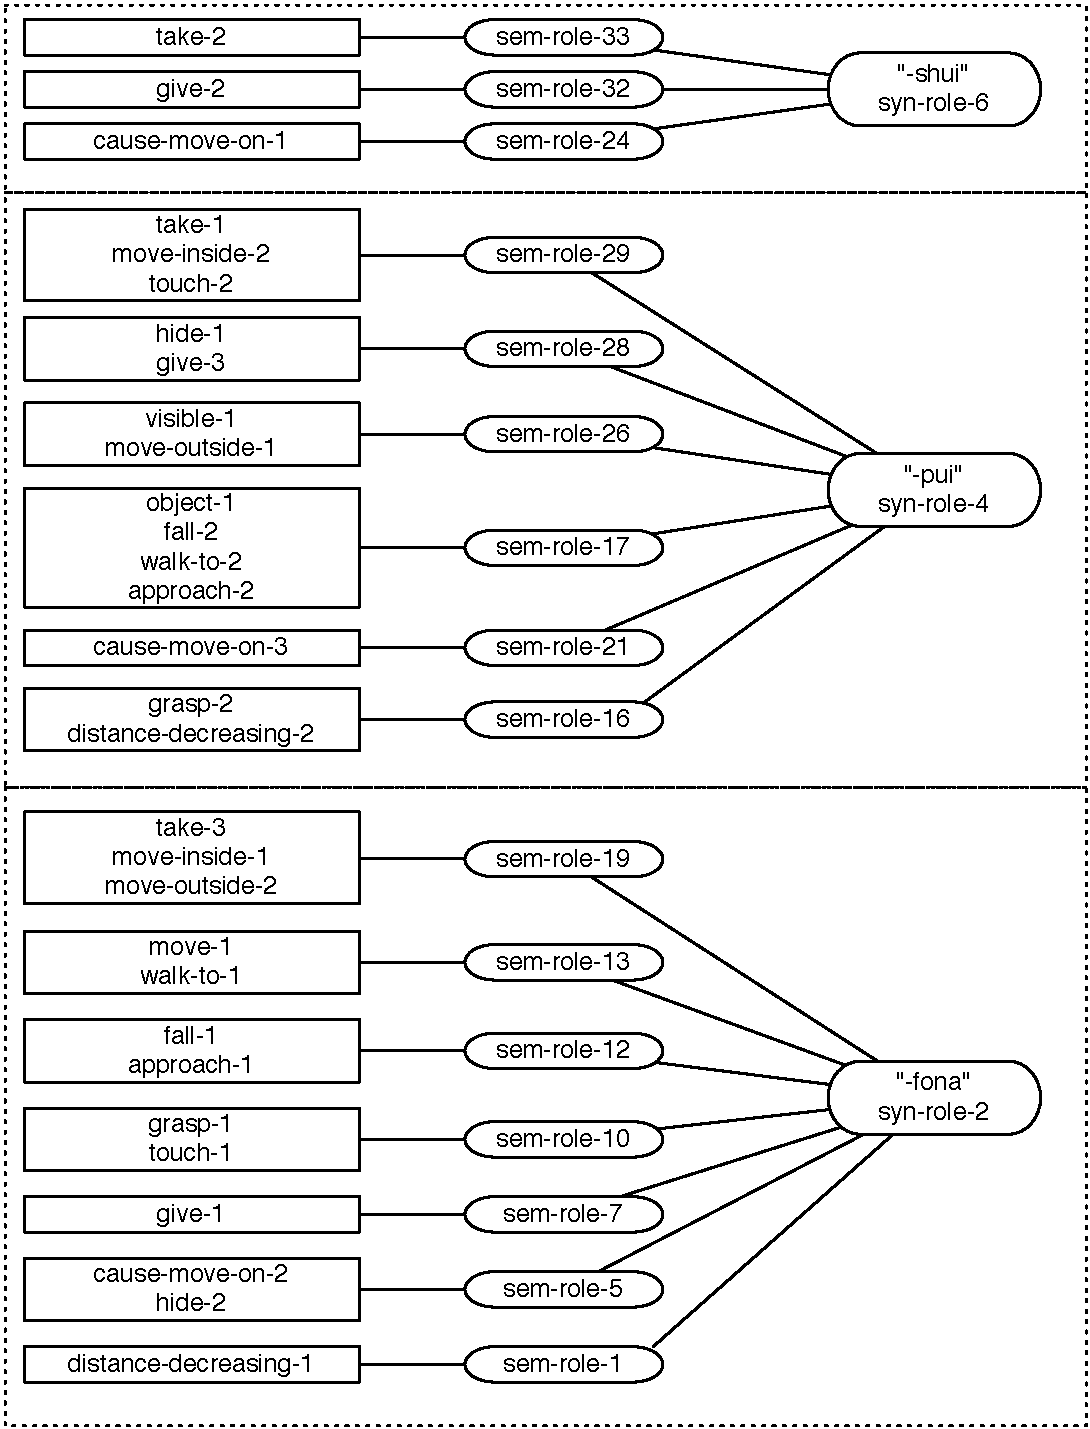
\includegraphics[width=0.9\textwidth]{Chapter4/figs/two-agent}}
  \caption[Syntactic roles: the mapping for two agents]{This diagram shows the mapping between participant roles and semantic roles; and between semantic roles and syntactic roles in the two-agent simulation on the emergence\is{emergence} of syntactic roles. Since there are no variation\is{variation}s in the simulation, both agents align their grammars perfectly. The results are taken as the baseline for the multi-agent simulations.}
   \label{f:two-agent}
\end{figure}


\subsubsection{Results}
 The two-agent simulation features no variation\is{variation} in the population\is{speech population} so the agents have no problems in aligning their grammars since they are endowed with the same algorithm of analog\is{analogy}ical reasoning. The resulting grammar is illustrated in Figure \ref{f:two-agent} which shows the mapping between participant, semantic and syntactic roles.

The diagram shows that the two agents indeed agree upon three case marker\is{case!case marking}s for covering all thirty participant roles. The results even seem to improve on the marker\is{case!case marking}s that were formed in baseline experiment 3a: ten semantic roles have been formed as opposed to six specific roles (which are also called `sem-roles' in the experiment for convenience's sake). On the other hand, the baseline experiment featured two semantic roles which covered six and four participant roles respectively, whereas the semantic roles in this case reach a maximum of four.

In terms of inventory size, the agents require 16 single-argument, 16 two-argument and 3 three-argument constructions. The fact that the number of two- and three-argument constructions is almost the same as in the experiments using no analog\is{analogy}y is due to the fact that only in two cases, a larger construction can also be fused with two different lexical entries. For example, {\em approach} and {\em fall} integrate with the same three constructions. So even though single-argument constructions can group several participant roles together, the patterns do not succeed in going beyond a verb\is{verb}-specific use.

The results of the two-agent simulation can now be taken as the baseline for the multi-agent simulations. A similar snapshot of the multi-agent simulation is presented in Figure \ref{f:multi-agent} and Figure \ref{f:multi-agent2}. These diagrams present the internal mappings between participant, semantic and syntactic roles from two different agents in the same population\is{speech population}. Both agents (as well as the other agents in the population\is{speech population}) converge on a coherent set of meaning-form mappings.

A closer look at the two diagrams shows that the agents have converged on five different case marker\is{case!case marking}s. Two of these marker\is{case!case marking}s are participant role-specific, while the others group together multiple roles. Compared to the two-agent simulation, there is a significant loss in number of semantic roles: the first agent has constructed five semantic roles and the second agent has constructed six semantic roles. This leaves 18 and 17 specific roles respectively. Most of the semantic roles also only cover two participant roles.
\begin{figure}[p]
\centerline{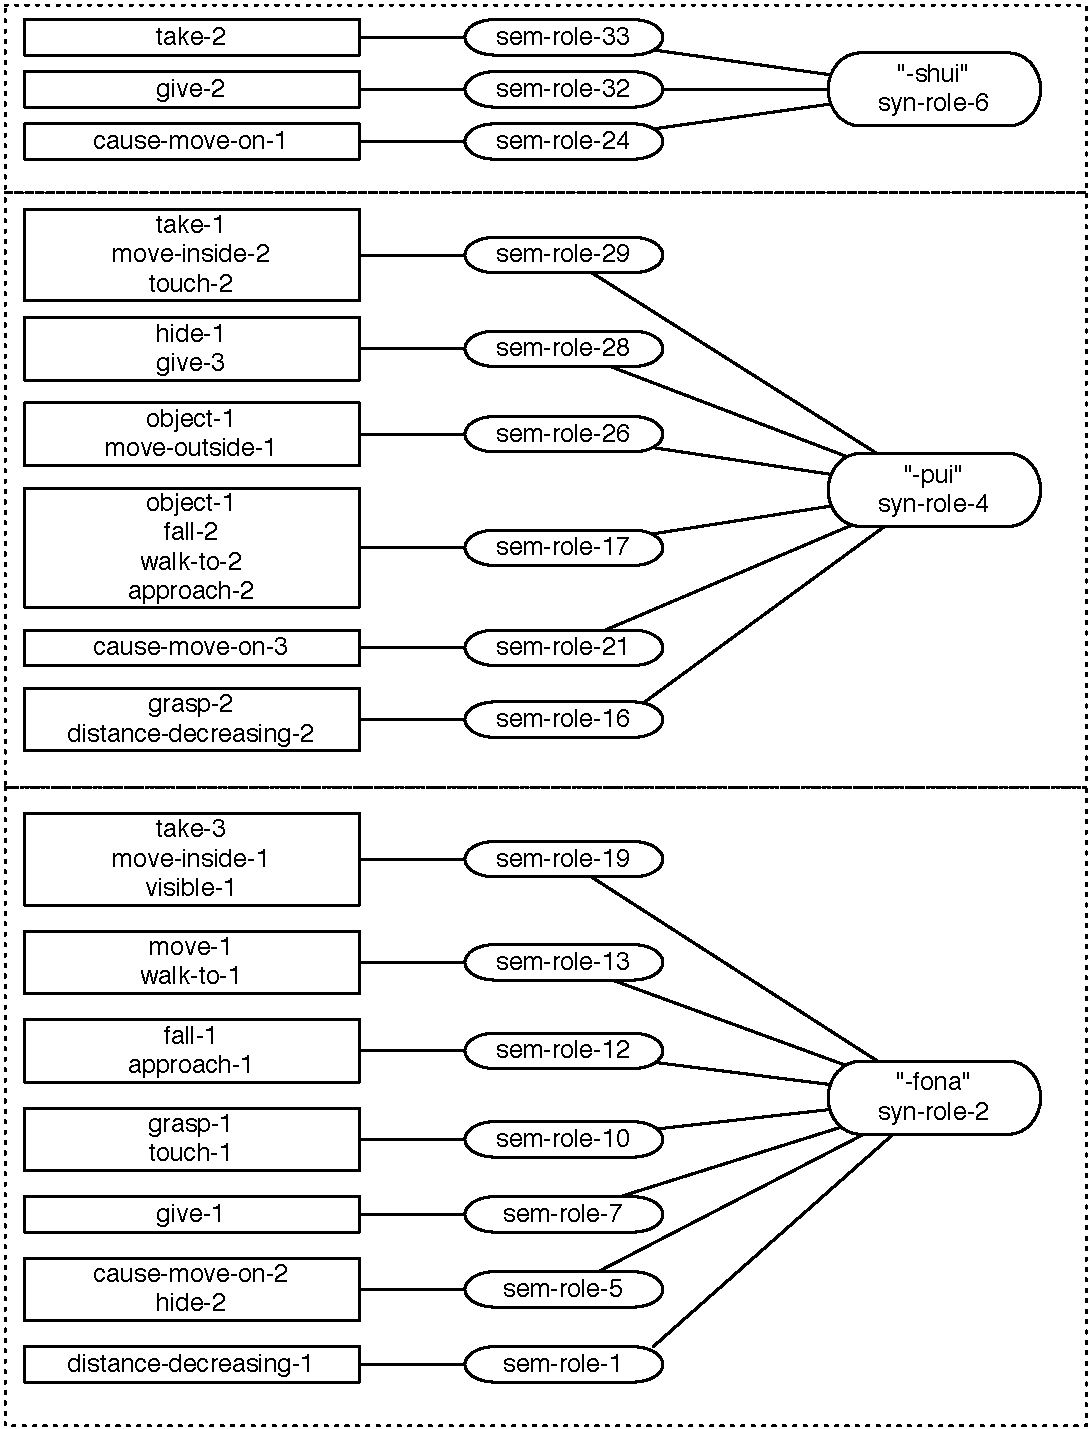
\includegraphics[width=0.9\textwidth]{Chapter4/figs/multi-agent}}
  \caption[Syntactic roles: the mapping for a single agent (1)]{The mapping between participant, semantic and syntactic roles in a single agent in the multi-agent simulation.}
   \label{f:multi-agent}
\end{figure}
\begin{figure}[p]
\centerline{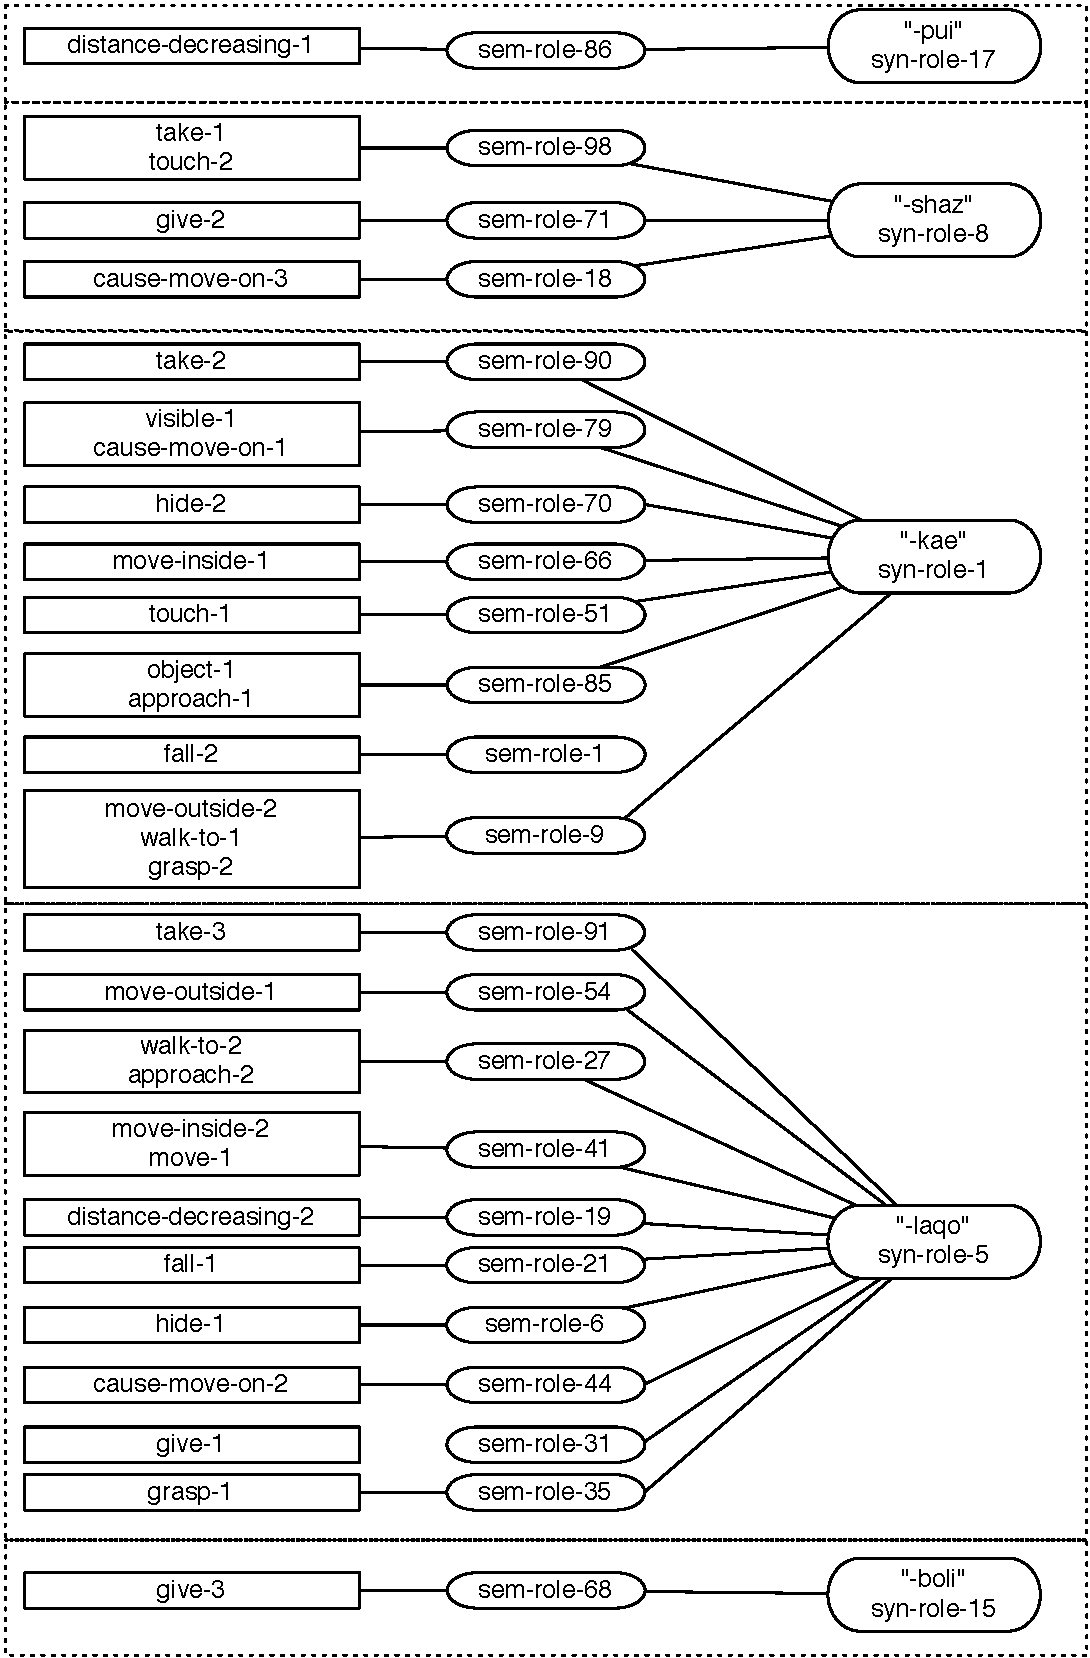
\includegraphics[width=0.9\textwidth]{Chapter4/figs/multi-agent2}}
  \caption[Syntactic roles: the mapping for a single agent (2)]{This diagram shows the internal mapping as known by another agent in the population\is{speech population}.}
   \label{f:multi-agent2}
\end{figure}

A comparison of the semantic roles of both agents also shows that they do not align their internal categorization. For example, the agent in Figure \ref{f:multi-agent} groups `move-outside-2', `walk-to-1', `fall-2' and `grasp-2' together. The other agent has a similar category but has constructed a separate role for `fall-2'. The other agent has also created a semantic role for covering `move-inside-2' and `move', whereas these are two distinct categories for the first agent.


\subsubsection{Discussion of the two-agent simulation}
 The agents in the two-agent simulation were capable of improving over baseline experiment 3a in terms of semantic roles, single-argument constructions and the number of marker\is{case!case marking}s. The improvement is due to the fact that the limited use of marker\is{case!case marking}s guides the search space more strongly during innovat\is{innovation}ion. In the previous experiments, each semantic role had its own case marker\is{case!case marking} so the chances that they had the same type frequency\is{type frequency}\is{frequency} were quite high. In this case, the speaker would always randomly choose which semantic role to exten\is{extension}d. In this new simulation, the type frequency\is{type frequency}\is{frequency} of the syntactic role was more important which led to a faster divergence between the productivity\is{productivity} rate of the cases. This means that semantic roles which would otherwise miss exten\is{extension}sion due to random choice now have more weight to categorize new participant roles.

An interesting side-effect of the innovat\is{innovation}ion algorithm is that there are two syntactic roles which cover almost exclusively semantic roles while a third role acts as a waste basket category for three participant roles which are all three part of events featuring three participants. This maps onto the distinction between agents and patients (and subject\is{syntactic role!subject}s and object\is{syntactic role!object}s) that is made by most of the languages in the world. Most theories of language assume a (near-)universal distinction between agents and patients to be given (either based on a universal conceptual space or on Universal Grammar\is{Universal Grammar}). This first tentative experiment suggests an alternative hypothesis: the distinction could emerge as a side-effect of communicative goals because language users want to make grammatically and communicatively relevant distinctions. In most of the cases, two or three syntactic roles suffice. The exten\is{extension}sion of case marker\is{case!case marking}s and the merger of semantic role could thus spontaneously lead to `core' cases.

A final remark considering the two-agent simulation is that there is no gain in terms of inventory size with respect to larger constructions. This is due to the fact that only a couple of constructions share the same semantic roles which combine into the same larger construction. As I suggested during the discussion of experiment 3, the newly formed patterns themselves should be considered by the analog\is{analogy}y as well. This could further increase the generalization and productivity\is{productivity} rate of the agents and could be an additional drive towards a prototypical agent-patient distinction.
\\
\\
\subsubsection{Discussion of the multi-agent simulation}
 The results of the multi-agent simulation shows that the alignment of an indirect and multilayered grammatical mapping is no trivial issue: the number of semantic roles constructed by each agent drops significantly and there are differences in how the internal mapping of each agent is organized. This is basically a problem of feedback: there is too much variation\is{variation} floating around in the population\is{speech population} for the agents to successfully retrieve the analog\is{analogy}y meant by the speaker. Additional feedback could consist of alternative agnat\is{agnation}ing structures that could be exploited for constructing semantic roles. This, however, would require the capacity of dynamically updating the function or meaning of the semantic roles, which the agents do not have (also see the concluding remarks in section \ref{s:base3}).

\subsection{The grammar square\is{grammatical square}: a roadmap for further work}
\label{s:future}

\begin{figure}[t]
\centerline{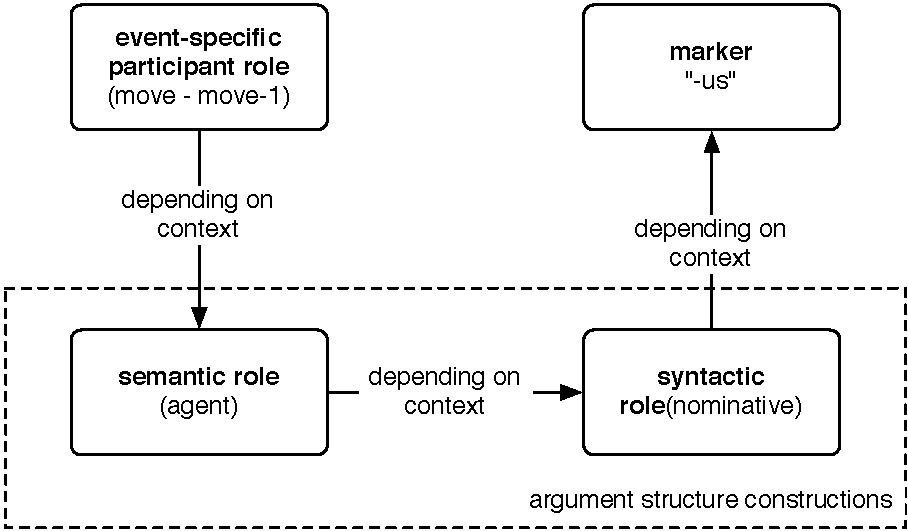
\includegraphics[scale=0.7]{Chapter4/figs/case}}
  \caption[The grammatical square\is{grammatical square}]{The grammar square\is{grammatical square} can be read as a roadmap for future research. Each mapping in the square is dependent on the context, so experiments should investigate which mechanisms and conditions can lead to such an indirect mapping.}
   \label{f:square-bis}
\end{figure}

The first experiments towards syntax showed that once the mapping between semantic roles and syntactic roles becomes indirect and polysemous, the agents are faced with a complex coordination problem\is{coordination problem}: the abstract layer of semantic and syntactic roles is not directly observable from the outside and the agents have no means of finding a shared categorization. Yet the alignment of this internal categorization is crucial in order to preserve a good productivity\is{productivity} and generalization rate for reaching communicative success\is{communicative success} in future interactions. In order to take this step, the experimental set-up needs to be expanded. We can use the grammar square (repeated in Figure \ref{f:square-bis}), as a guidance for identifying which efforts need to be made in order to solve this coordination problem.


\subsubsection{Mapping participant roles onto semantic roles}
 Participant roles of a particular event can map onto several semantic roles in natural languages. This is clear in the following sentences, in which {\em the window} first plays the role of patient, then some entity which undergoes a change of state, and finally some stative entity:

\ea
He broke the window.
\label{e:aspect-1}
\item The window broke.
\label{e:aspect-2}
\item The window was broken.
\label{e:aspect-3}
\z

In the experiments presented in this book, such functional variation\is{variation} was impossible: during conceptualization\is{conceptualization}, the agents always profile \is{event profile}the complete participant role in the event structure\is{event structure}. This could lead to sentences similar as example \ref{e:aspect-1}. However, in the other two sentences, only a subpart of the participant role is profiled\is{event profile}: example \ref{e:aspect-2} profiles the change of state whereas example \ref{e:aspect-3} profiles the resulting state of the participant.

In order to achieve the same functional variation\is{variation}, the agents would thus have to be able to include aspect\is{aspect} (and tense\is{tense}) distinctions in their conceptualization\is{conceptualization}. For this, the conceptualization\is{conceptualization} algorithm and the algorithm for analog\is{analogy}y would have to be changed in order to include the hierarchical structure of the event descriptions and the time stamps provided by the event recognition\is{event recognition} system. On the level of the interaction pattern, the agents would somehow have to be able to get sufficient feedback in order to recognize and learn the relevant aspect\is{aspect}ual distinctions. The emergence\is{emergence} of grammatical marker\is{case!case marking}s for aspect\is{aspect} (and tense\is{tense}) is no trivial matter and goes well beyond the scope of this book.


\subsubsection{Mapping semantic roles onto syntactic roles}
 The mapping between semantic roles and syntactic roles can already be multilayered in nature without taking information structure\is{information structure} into account: in examples \ref{e:aspect-2} and \ref{e:aspect-3}, the distinction is not one of active\is{construction!active construction} versus passive\is{construction!passive construction}, but rather one of aspect\is{aspect}. In order to see such alternations emerging, the idea of reuse\is{reuse} can be exploited again. As the agents develop their grammars, they increase their expressive power. From the moment they want to express aspect\is{aspect}ual distinctions as well, they could try to reuse\is{reuse} the existing grammatical system instead of inventing some new strategy. This puts pressure on the existing convention\is{convention}s and may lead to additional abstraction\is{abstraction}s in the form of syntactic roles.

Another way to investigate the emergence\is{emergence} of syntactic roles would be to endow the agents with the capacity of dynamically updating the representation of their categories. If categories are not fixed but dynamic, there is a risk of `category leakage\is{category leakage}' as observed in natural languages: some categories start expanding their use which could lead to the merger of two semantic roles into one case. Typically, the more frequent cases would start exten\is{extension}ding their usage which could gradually lead to prototypical agent and patient categories.


\subsubsection{Mapping syntactic roles onto case marker\is{case!case marking}s}
 In the experiments, there is a one-to-one relation between syntactic roles and case marker\is{case!case marking}s. In natural case grammar\is{case!case grammar}s, however, there are often paradigms\is{case!case paradigm} of related marker\is{case!case marking}s that together cover a particular case. These marker\is{case!case marking} alternations typically indicate grammatical distinctions in terms of gender\is{gender} and number\is{number}. Evolving this kind of variation\is{variation} would thus require a need for marking grammatically relevant distinctions between arguments.

Even more intriguing are case systems\is{case!case system} where the same marker\is{case!case marking}s can be used to indicate different cases. For example, Latin\is{Latin} uses the inflection\is{inflection} {\em -um} to mark nominative case in neuter singular\is{number!singular} words ({\em bellum} `war') and accusative case in masculine singular\is{number!singular} words ({\em dominum} `master') \citep[4--5]{blake94case}. This means that case marker\is{case!case marking}s somehow manage to grow a paradigmatic\is{case!case paradigm} case system\is{case!case system} which goes beyond the borders of individual cases. Applied to the experiments, this would mean lifting the present assumption\is{assumption} that competing case marker\is{case!case marking}s are always competing with each other for marking a particular participant role. Instead, agents should be allowed to accept competit\is{competition}ion and variation\is{variation} at each possible mapping in the grammatical square\is{grammatical square}. This may lead to a credit assignment problem\is{credit assignment problem} in which the agents can never have complete certainty about which mapping in the grammatical square\is{grammatical square} was relevant during a particular innovat\is{innovation}ion.

From the above discussion it should be clear that scaling up the experiments towards richer syntax and grammar is not a trivial matter. It would include research into the emergence\is{emergence} of aspect\is{aspect} and tense\is{tense} distinctions, a dynamic representation of linguistic categories, and allowing competit\is{competition}ion on all aspects of the grammatical square\is{grammatical square}. A scale-up to include information structure\is{information structure} as well would involve expansion of the language game\is{language game} model to larger dialogue\is{dialogue}s, which creates the need for additional capacities such as episodic memory\is{episodic memory}, scoping and coordination issues and possibly anaphora resolution\is{anaphora resolution}.